\documentclass[double,10pt] {beavtex}
% \usepackage[margin=1.5in,footskip=1.5in]{geometry}

\usepackage{natbib}
\usepackage{amsmath} %
\usepackage{xcolor}
\usepackage{color}
\usepackage{array}
\usepackage{wrapfig}
\usepackage{multirow}
\usepackage{tabularx}
% \usepackage{color, colortbl}
% \definecolor{name}{system}{definition}
% \definecolor{Gray}{gray}{0.9}
\usepackage{graphicx}
\graphicspath{ {./images/} }
% \usepackage[demo]{graphicx}
\usepackage{subcaption}
\usepackage[utf8]{inputenc}
\usepackage[T1]{fontenc}
\usepackage{microtype}
\usepackage{enumitem}
\usepackage{lipsum}
\usepackage{url}
\usepackage{lambda} %
\usepackage{listings}
\usepackage{indentfirst}
% \usepackage{hyperref}
\usepackage[hidelinks]{hyperref}

% use \term for introducing new terms
\newcommand{\term}[1]{\textit{#1}}
\newcommand{\ChcL}{\OB{\langle}}
\newcommand{\ChcR}{\OB{\rangle}}
\newcommand{\Chc}[3][f]{\OB{#1\langle#2,#3\rangle}}
\newcommand{\Opt}[2][f]{\OB{#1\langle#2\rangle}}
\newcommand{\ChcPP}[3][f]{\Chc[#1]{\prog{#2}}{\prog{#3}}}
\newcommand{\Step}{\OB{\;\mapsto}\;}

% macro to select a scaled-down version of Bera Mono (for instance)
\makeatletter
\newcommand\BeraMonottfamily{%
  \def\fvm@Scale{0.85}% scales the font down
  \fontfamily{fvm}\selectfont% selects the Bera Mono font
}
\makeatother

% \lstset{
%   basicstyle=\linespread{1}\ttfamily\small, frame=single,numbersep=10pt,
% }

\lstset{
  basicstyle=\linespread{1}\fontsize{9}{10}\selectfont\BeraMonottfamily, frame=single,numbersep=10pt,aboveskip=12pt
}

% citation groups
\newcommand\CCcore{EW11tosem,Walk13thesis,HW16fosd}
\newcommand\VPcore{EW11gttse,CEW16ecoop}
\newcommand\VPstretch{WE12gpce,EWC13fosd}
\newcommand\VPdata{Walk14onward,MMWWK17vamos,SE17fosd}
\newcommand\VPfacets{AF:POPL12,YYS12,Aus13,Sch16,Austin14, Pretnar15}
\newcommand\VPmultiexec{DP10,JR11,deG14,Kwon16,RS16,Kammar2013,Plotkin2001}
\newcommand\VPaware{NKN:ICSE14,Ngu15,MWKTS:ASE16}
% \newcommand\VEff{Pretnar15}

% cite later: Sch16 -- faceted execution in Haskell

\title{Integrating Side Effects in Variational Programs Using Algebraic Effects}
% \title{Handling Effects in Variational Programs}
\author{Ghadeer Alkubaish}
\degree{Master of Science}
\doctype{Thesis}
\department{Electrical Engineering and Computer Science}
\depttype{School}
\depthead{Director}
\major{Computer Science}
\advisor{Eric Walkingshaw}
\submitdate{Feb 24, 2020}
\commencementyear{2020}

\abstract{
Variational programming supports efficiently executing many related programs at once by encoding all of the programs in one "variational program" that captures the differences among them statically and explicitly. An open problem in variational programming is how to handle side effects---if two program variants perform different side effects, we cannot separate the effect of one variant from the other since the outside world is not variational. A potential solution is to create variation-aware execution environments for variational programs, for example, a variational file system that keeps track of file variants corresponding to program variants. However, it is infeasible to do this for all kinds of effects. Also, there are different ways to handle the interaction of effects and variation that are incompatible with each other, preventing a one-size-fits-all solution.

In this thesis, we argue that \term{algebraic effects} can be used to resolve the problem of combining variation and effects by enabling programmers to flexibly and incrementally extend a variational programming environment to handle new kinds of effects. We present a proof-of-concept prototype in the \emph{Eff} programming language that demonstrates how a variational programming environment can be extended to support file input/output. Crucially, such extensions are done at the library level, which enables handling new kinds of effects and handling existing effects in multiple ways, both of which are essential in variational programming applications.
}
% \acknowledgements{}
\acknowledgements{

First and foremost, I thank my God for all the blessings in my life.

Then, I would like to thank my wonderful loving husband Ali who has always been for me in my rough and good times. Ali became my family and best friend in my life away from home. He believed in me and did all he could to let me achieve my goals. I thank him for all support, understanding and encouragements. He is the one secret behind every success I make or challenge I overcome. 

I thank my two adorable sons Hassan and Rida for being in my life - making it joyful, exciting and a bit more busy! 

I thank my loving family: Mom, Dad, Sisters and Brothers. I appreciate that they are always standing up for me during all of my milestones, pushing me hard, trusting me, and cheering for every success I make. My special thanks to my great super Mom. She is the one person who believes in me the most. I thank her for your prayers, love and constant communication regardless of the time difference and long distance. I do what I do to make her proud. 

I thank my great advisor Professor Eric Walkingshaw. I thank his high confidence in me, his inspiring words throughout my journey and his powerful encouragement which kept me going. I honor his time, lessons, feedback and enthusiasm. I appreciate his understanding and accommodations for my special needs and restricted schedule. I appreciate his respect to my values. I give him all the credit for me continuing my studies and accomplishing this work.

I thank Professor Martin Erwig who has been a main source of knowledge in the PL group. I appreciate everything I learned from him through classes or the reading group.

My very special thanks to my mentor Jed Irvine for the great sessions in improving my technical writing. He has effectively improved my skills, reviewed my paper, and gave me the time and effort I needed with great generosity.

I thank my PL research mates for the reading group meetings where we exchanged many great ideas. I specially thank my group mates Jeff, Parisa, Fariba and Qiaoran. I appreciate all of their feedback during the writing workshops. 

I thank the great faculty members of OSU who I learned from or worked with. I thank Professor Prasad Tadepalli who I enjoyed working with on the GTA assignment project. I thank Professor Jennifer Parham-Mocello who has always shown love and support. I thank the adviser Calvin Hughes for his unlimited advising and support.

I thank Professor Glencora Borradaile for her support and empathy. I will absolutely miss my many stops by her office. She has always helped me through my difficult times in personal and graduate life.

I thank my very special friend Mahsa for her exceptional support, especially after moving out from Corvallis and starting to commute. I thank her for always checking on me, hosting me in your apartment during lunch time and cooking for me. In my hardest days during pregnancy and commuting, Mahsa has been there for me.

I thank my friends in Corvallis and Portland. I appreciate all of the great times we spend together. I thank my very special extended family who always provide me with love and support.

I thank OSU for the GTA position which provided me with teaching skills and secured me financially. I also thank SACM for the scholarship which provided financial stability plus child care support.

I thank my committee members---Eric Walkingshaw, Martin Erwig, Arash Termehchy, and Vergara Hector for their time, willingness to evaluate my work, and feedback.
}

\begin{document}
\maketitle
\mainmatter

\chapter{Introduction}
\label{sec:introduction}
\term{Variational programming} \cite{\VPcore} is an emerging paradigm for representing and computing with explicit variation in code and data.
%
It is a generalization of the ideas underlying \term{faceted execution} \cite{\VPfacets} for enforcing dynamic information-flow security and \term{variability-aware execution} \cite{\VPaware} for testing software product lines, and has a range of other applications across computer science such as model checking \cite{Cla10}.
%
However, integrating side effects (e.g. state updates, exceptions, file I/O, standard input/output, and database queries) in variational programs is challenging because the execution environment of these programs is not variational. Therefore, we cannot separate the effect of one variant from the other which causes effects to be performed in wrong contexts (the words effect and side effect are interchangeably used in this thesis).

In this thesis, we argue that \term{algebraic effects} can be used to resolve the problem of combining variation and effects by enabling programmers to extend variational programming environments to handle new kinds of effects or handle existing effects in different ways. We present a proof-of-concept prototype in the \emph{Eff} programming language that demonstrates how the variational programming environment can be extended to support file input/output. 
%

In this chapter, we discuss the insight, formalization, and execution of variational programming. We show the challenge of integrating variational programming with side effects. 
%
We explore various approaches in overcoming these challenges and discuss their limitations.
%
We discuss our solution and its advantages and drawbacks.
%
Finally, we outline the contributions of this work.

A core insight of variational programming is that the execution of sets of related programs, and/or execution over sets of related data, can be made faster by computing over a \emph{single variational artifact} that shares common parts while capturing differences through localized, explicit \emph{variation points}. To illustrate this insight, consider the three related programs which calculate the flight cost for different types of tickets in a booking system and the corresponding \textbf{variational flight cost} program in Figure \ref{fig:vp_eg}. We assume tickets come in three categories: \textbf{Economy}, \textbf{Business} or \textbf{First}. Also, there are \$55 flight fees and a \$45 booking fee added to the cost. In each case, the price is calculated by summing up the price per ticket with the total fees.

\begin{figure}[h]
    \centering
\begin{minipage}[t]{0.49\textwidth}
\textbf{\underline{Economy}} \\
\texttt{let ecoPr =  \$649;;}\\ 
\texttt{let cost = }\\
$\texttt{ \quad 55 + 45 + ecoPr;;} \\$
\end{minipage}
\begin{minipage}[t]{0.49\textwidth}
\textbf{\underline{Business}} \\
\texttt{let busPr =  \$3955;;}\\
\texttt{let cost = }\\
$\texttt{ \quad 55 + 45 + busPr;;} \\$

\end{minipage}
\hfill

\begin{minipage}[t]{0.49\textwidth}
\textbf{\underline{First}} \\
\texttt{let fstPr =  \$5812;;}\\
\texttt{let cost = }\\
$\texttt{ \quad 55 + 45 + fstPr;;} \\$

\end{minipage}
\begin{minipage}[t]{0.49\textwidth}
\textbf{\underline{Variational flight cost}} \\
\texttt{let vTicketPr = }\\ 
$\texttt{ \quad \Chc[\texttt{Economy}]{\texttt{\$649}}{\Chc[\texttt{Business}]{\texttt{\$3955}}{\texttt{\$5812}}}}$\\
\texttt{let vCost = }\\
$\texttt{ \quad 55 + 45 + vTicketPr;;} \\$
\end{minipage}\\

\caption{Variational flight cost.}
  \label{fig:vp_eg}
\end{figure}
%
 The value $\Chc[\texttt{Business}]{\texttt{\$3955}}{\texttt{\$5812}}$ represents a \term{choice} between the alternatives $\texttt{\$3955}$ and $\texttt{\$5812}$ (this choice is nested in another choice). The \term{condition} of the choice is an \term{option} \texttt{Business}, which may be either enabled (true), disabled (false), or open. A choice is similar to a conditional expression (if-then-else), except that if its condition is open, it represents \term{both} alternatives at the same time. Multiple choices with the same condition will always be synchronized while choices with conditions based on different options may vary independently. 
 
Enabling or disabling a choice is what we call \term{selection}. To select the left alternative of the choice \texttt{vTicketPr}, we say (\texttt{selectV Economy vTicketPr}). This returns {\texttt{\$649}}. To select the right alternative of it, we say (\texttt{selectV (!Economy) vTicketPr}). 
%
This returns {\Chc[\texttt{Business}]{\texttt{\$3955}}{\texttt{\$5812}}}. An open selection (\texttt{selectV true vTicketPr}) selects both alternatives, so this returns \texttt{vTicketPr}. The notation and semantics of choices is a previous work on the \term{choice calculus}~\cite{EW11tosem,Walk13thesis,HW16fosd}.

We can extend the evaluation semantics of our programming language to include choices by simply mapping over their alternatives. This allows us to evaluate \texttt{vCost} to the following choice with the following sequence of reduction steps.
%
\begin{align*}
\underline{\texttt{55+45+\Chc[\texttt{Economy}]{\texttt{649}}{\Chc[\texttt{Business}]{\texttt{3955}}{\texttt{5812}}}}}\\
~\Step~ & \texttt{\underline{55+45} + \Chc[\texttt{Economy}]{649}{\Chc[\texttt{Business}]{\texttt{3955}}{\texttt{5812}}}} \\
~\Step~ & \texttt{100 + \underline{\Chc[\texttt{Economy}]{\texttt{649}}{\Chc[\texttt{Business}]{\texttt{3955}}{\texttt{5812}}}}} \\
~\Step~ & \texttt{\Chc[\texttt{Economy}]{\underline{\texttt{649+100}}}{\Chc[\texttt{Business}]{\texttt{3955+100}}{\texttt{5812+100}}}} \\
~\Step~ & \texttt{\Chc[\texttt{Economy}]{\texttt{749}}{\underline{\Chc[\texttt{Business}]{\texttt{3955+100}}{\texttt{5812+100}}}}} \\
~\Step~ & \texttt{\Chc[\texttt{Economy}]{\texttt{749}}{\Chc[\texttt{Business}]{\underline{\texttt{3955+100}}}{\texttt{5812+100}}}}  \\
~\Step~ & \texttt{\Chc[\texttt{Economy}]{\texttt{749}}{\Chc[\texttt{Business}]{\texttt{405}5}{\underline{\texttt{5812+100}}}}}  \\
~\Step~ & \texttt{\Chc[\texttt{Economy}]{\texttt{749}}{\Chc[\texttt{Business}]{\texttt{4055}}{\texttt{5912}}}}
\end{align*}
%
This reduction process represents \term{variational execution} which dynamically evaluates all variants of a program, but observe that we only visited the expression $\texttt{55 + 45}$ once rather than three times if we had evaluated the three programs separately.
%
Although the saving here is small, it adds up as the size of shared programs and the number of independent options increases.
%
In fact, many applications of variational programming involve efficiently computing or exploring an exponential number of variants by exploiting the ideas of capturing variation locally (e.g.\ in choices) and sharing common parts of data and computations. 

\begin{wrapfigure}{r}{0.25\textwidth}
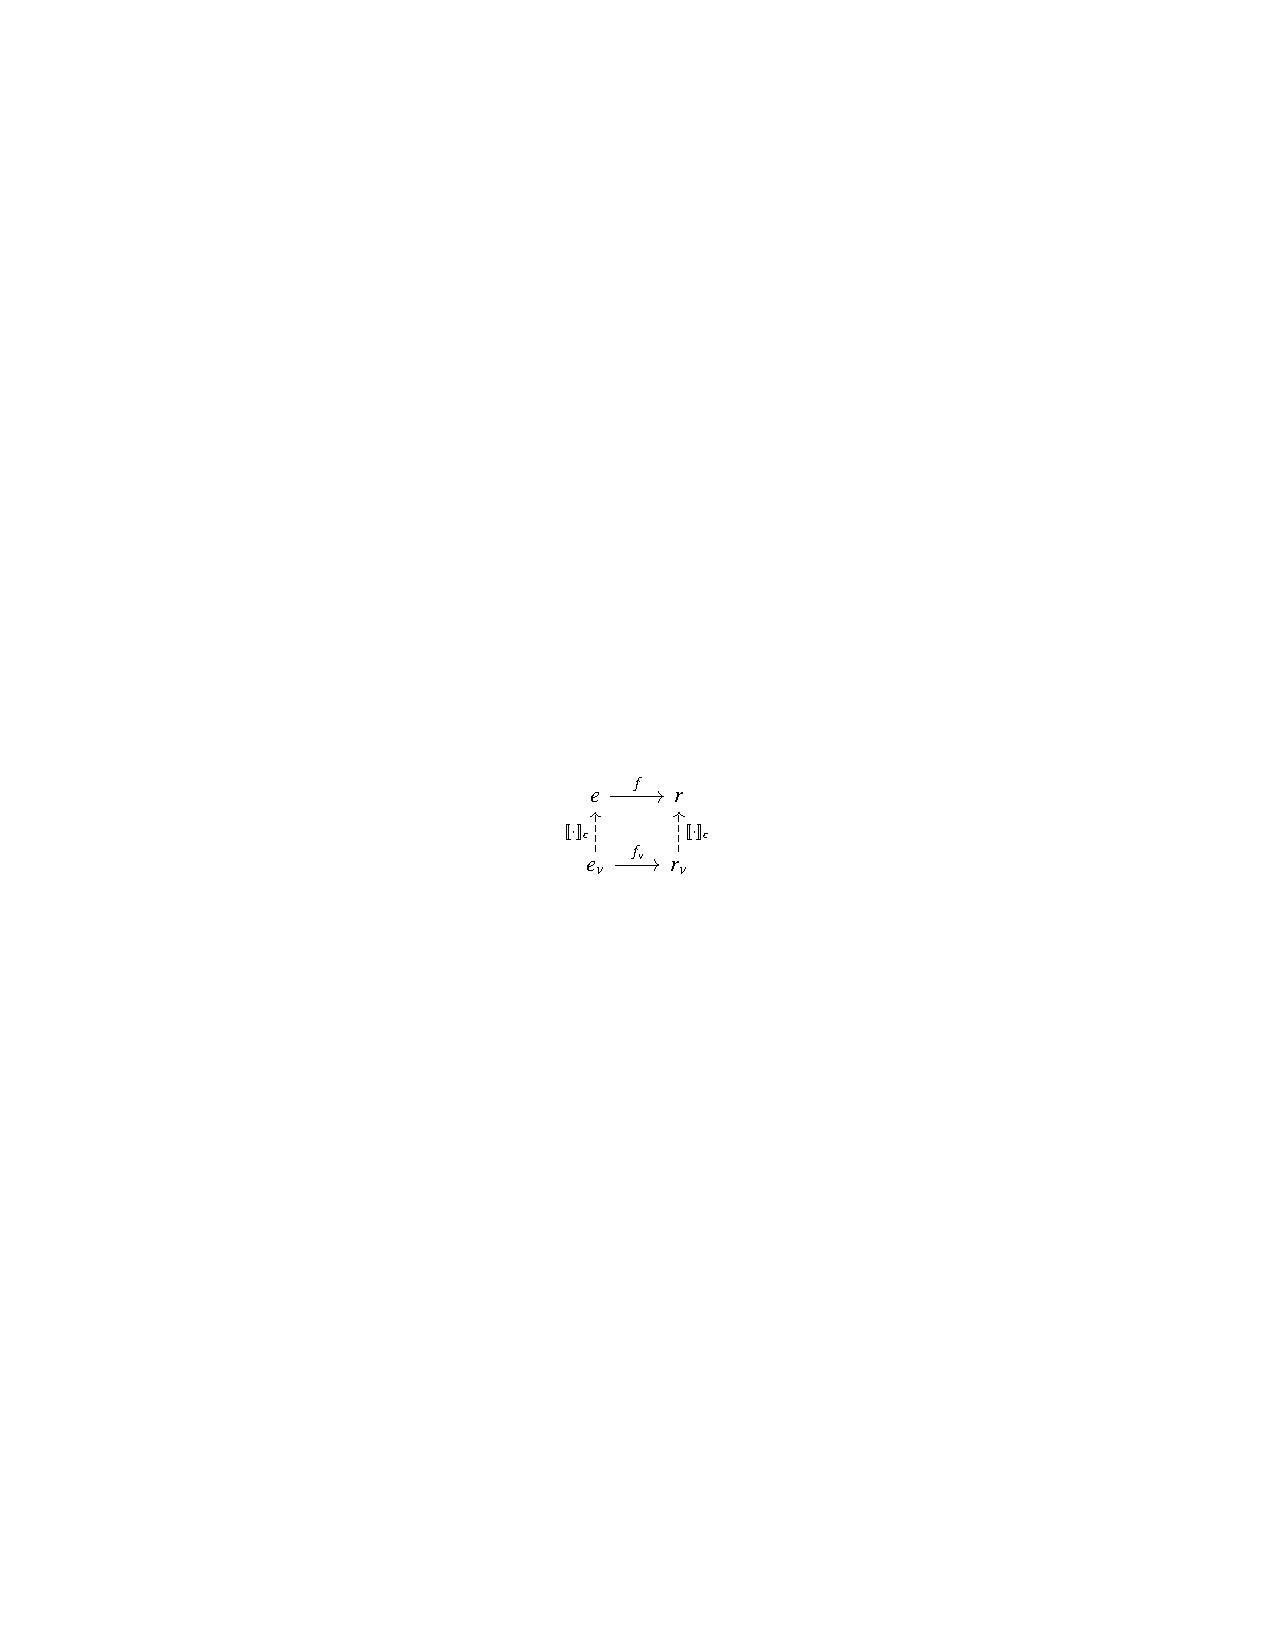
\includegraphics[width=0.9\linewidth]{figures/diagram.pdf} 
\end{wrapfigure}

When mapping analyses or computations over variational terms, the crucial property
that is maintained is \term{variation preservation} \cite{CEW16ecoop}. This is illustrated by the commuting
diagram at right, where \texttt{f} is a plain function that transforms a plain expression \texttt{e} into a plain result \texttt{r}, and $\texttt{f}_\texttt{v}$ is the corresponding \term{variational function} that transforms the variational expression $\texttt{e}_\texttt{v}$ into a variational result $\texttt{r}_\texttt{v}$. The operation $[\![.]\!]_{\texttt{c}}$ refers to the select operation mentioned above; for example, $[\![\texttt{e}_\texttt{v}]\!]_{\texttt{c}}$ is equivalent to \texttt{select c $\texttt{e}_\texttt{v}$ = e}
% selects from  $\texttt{e}_\texttt{v}$ with option \texttt{c}, yielding \texttt{e}. 
The variation-preservation property states that $\texttt{f}_\texttt{v}$ is exactly equivalent to running \texttt{f} on every plain variant of $\texttt{e}_\texttt{v}$. That is, we obtain the same plain result \texttt{r} by either $\texttt{f}([\![\texttt{e}_\texttt{v}]\!]_{\texttt{c}})$ or $[\![\texttt{f}_\texttt{v}(\texttt{e}_\texttt{v})]\!]_{\texttt{c}}$, for any option \texttt{c}.

Now, consider adding side effects to a variational program. For example, someone might like to write the variational flight cost calculated in Figure \ref{fig:vp_eg} into a file as shown below. 
%
\begin{lstlisting}[escapeinside={(*}{*)}]
#WriteFile "flight.txt" ("The total flight cost:");
#WriteFile "flight.txt" ("$" + (* \Chc[\texttt{Economy}]{\texttt{"749"}}{\Chc[\texttt{Business}]{\texttt{"4055"}}{\texttt{"5912"}}}*))
\end{lstlisting}
%
With the current implementation of variational execution, every choice alternative would be visited. Hence, side effects that occur in choices would be performed during the process even in the alternative context. To see how this is an issue, look at the following output of the program above. 
%
\begin{lstlisting}
The total flight cost: 
$749
4055 
5912
\end{lstlisting}
%
This program writes the text of each variant while the desired behavior is to only write the text of the corresponding variant. Variational programming uses variational data-structures to manage different variants and separate their results, but the current environments of the effects we work with are not variational, so we can not separate their variants which causes this problem.

There are several solutions to allow working with side effects in variation. One possible solution is to make a variation-aware interface for every effect type we work with, that is a variational file system, database \cite{ATW17dbpl} and so on. Thus, if the file system was variational, there would be conceptually a different file instance for every new option introduced by a choice as shown below.\\

\begin{minipage}{0.3\textwidth}
\textbf{\underline{Economy.txt}} \\
\texttt{The total flight cost: }\\
\texttt{\$749}\\
\end{minipage}
\begin{minipage}{0.3\textwidth}
\textbf{\underline{NotEconomyBusiness.txt}} \\
\texttt{The total flight cost: }\\
\texttt{\$4055}\\
\end{minipage}
\begin{minipage}{0.3\textwidth}
\textbf{\underline{NotEconomyNotBusiness.txt}} \\
\texttt{The total flight cost: }\\
\texttt{\$5912}\\
\end{minipage}\\
\hfill\\
%
As we introduce more options, more instances should be created. However, making a special variational infrastructure for every effect type is very complex, infeasible or incompatible in some domains. Another solution is to avoid variational execution from running side effects when they occur in variation, but this would cut their useful applications.
% Therefore, we propose a library level solution which allows programmers to work with effects in variational programs.

In this thesis, we argue that algebraic effects can be used to resolve the problem of combining variation and effects by enabling programmers to flexibly and incrementally extend variational programming environments to handle new kinds of effects or handle existing effect differently. We present a proof-of-concept prototype in the \emph{Eff} programming language. We implement variation as an algebraic effect and then demonstrate how the variational programming environment can be extended to support file input/output. Given that there is not a comprehensive solution for all effects, this approach is the best given the constraints. It allows programmers to work with effects on a case-by-case basis by building new libraries to handle them. Unfortunately, implementing variation as an effect is not efficient as the number of options increases. Therefore, we argue that having built-in features in the programming language itself for working with variation would be more effective.

This work includes the following contributions. 
%
\begin{itemize}
  \item We implement variation as an effect and show examples of how it works (Chapter \ref{sec:Variational_exe}). We show the limitations of this implementation when we start to integrate side effects in variational programs (Chapter \ref{sec:Variational_effects}). Our approach in addressing these limitations is by writing new handlers for the variation effect to work with interaction of variation and effects on a case-by-case basis using algebraic effects. As a proof-of-concept, we write new handlers to support file writing (Chapter \ref{sec:file_IO_writing}) and reading (Chapter \ref{sec:file_IO_reading}) which are hard to work with otherwise. As part of this, we also extend text files with a variation encoding (Chapter \ref{sec:file_format}).
  \item We introduce an abstract variational queue that can be used in different variational programming applications (Chapter \ref{sec:queue_lib}). We use the variational queue to represent variational files as part of our proof-of-concept. 
  \item We discuss the limitations of implementing variation as an effect (Chapter \ref{sec:efficiency}).
\end{itemize}
Our prototype implementation is publicly available at the GitHub repository VEffect\footnote{https://github.com/lambda-land/VEffect}. 



\chapter{Background: Algebraic Effects}
\label{sec:background}
\begin{figure}[!htb]
  \centering
  \begin{lstlisting}[linewidth=.9\textwidth]
effect Get: unit -> int;;
effect Set: int -> unit;;

let state = handler
  | val y -> (fun _ -> y)
  | #Get () k -> (fun s -> k s s)
  | #Set s' k -> (fun _ -> k () s')
  | finally g -> g 0
;;
\end{lstlisting}
  \caption{The integer state effect and handler.}
  \label{fig:state-effect}
\end{figure}
%
As background, we introduce \term{algebraic effects} - what they mean and how to use them - by showing a code example. The programming language used in this work is called \term{Eff}\footnote{https://www.eff-lang.org/} which is based on the programming language \emph{OCaml} and has similar syntax and features \cite{Pretnar15}. \emph{Eff} has a flexible extensible effect system that does not exist in \emph{OCaml} called \term{algebraic effects} which is the main tool used in our work (the words effects and algebraic effects are interchangeably used in this thesis). We use \emph{Eff} syntax throughout this thesis in our coding examples. 

\emph{Eff} is based on algebraic effects and handlers. An effect is defined by a set of primitive operations (e.g. \term{set} and \term{get} for a \term{state} effect) and implemented by one or more handlers. The fact that multiple handlers can be written for the same effect increases the power and flexibility of this system. Algebraic effects expand on the traditional exception handling mechanism by allowing computational effects to be thrown and caught by a handler that performs certain computation. Thrown effects have a continuation parameter that could be invoked with an argument of the thrown effect's return type. The continuation resumes the execution from the point where the effect operation was thrown.  

To get a sense of how algebraic effects are used and defined, refer to the integer state effect \cite{Pretnar15} in Figure \ref{fig:state-effect}. This state effect has two primitive operations \texttt{\#Set} and \texttt{\#Get} declared with the keyword \texttt{effect}. \texttt{\#Get} takes a unit value and returns the corresponding state value. \texttt{\#Set} takes a new state value and returns a unit value.

The handler has a separate case for each effect operation plus the return and action cases. The continuation parameter \texttt{k} in \texttt{\#Set} and \texttt{\#Get} is invoked with values of the return type; in \texttt{\#Get} the return type is \texttt{int} and in \texttt{\#Set} the return type is \texttt{unit}. The result of each continuation invocation (\texttt{k ()} or \texttt{k s}) is a function that takes a parameter of type \texttt{int} corresponding to the current state value, which in the case \texttt{finally} gets its initial value 0. In the case of \texttt{\#Get}, the handler returns a function that invokes the continuation with current state value and passes it unchanged to the result of the continuation. In the case of \texttt{\#Set}, the handler returns a function that invokes the continuation with a unit value and passes the new state value (the parameter of \texttt{\#Set}) to the result of the continuation. The \texttt{finally} case starts the computation with the initial value \texttt{0}. The \texttt{val} case is the return case. 
%

Note that we establish the handler scope for a given expression using the following syntax.
%
\[
\texttt{with handler\_name handle expression}
\]
%
Any effect operation that occurs within that code block will be within the bound of the \texttt{state} handler instance. 
\begin{lstlisting}
with state handle
    #Set(5); #Set(#Get() + 1); #Get()
;;
\end{lstlisting}
%
This code sets the state to \texttt{5}, then increments it by \texttt{1}. Then, evaluates the state again with the effect operation \texttt{\#Get}, which gives the result of \texttt{6}. 

\chapter{Variation as an Algebraic Effect}
\label{sec:Variational_exe}
\begin{figure}[!htb]
  \centering
\begin{lstlisting}[]
effect Choice : ctx -> bool;;

let v_handler = handler
    | #Choice s k -> 
        let l = select s (k true) in
        let r = select (Not s) (k false) in
	    prepend s l @ prepend (Not s) r
    | val x -> [(Lit true,x)]
;;

let chc d l r = if #Choice d then l else r;;
\end{lstlisting}
  \caption{The variation effect and handler.}
  \label{fig:choice-impl}
\end{figure}
%
We use the algebraic effects system introduced in Chapter \ref{sec:background} to implement variation as an effect. We use it as part of our proof-of-concept for the integration of variation and side effects. However, implementing variation as an effect is not efficient when the number of options increases. We discuss the limitation of this implementation in Chapter \ref{sec:efficiency}. 

In this chapter, we show the algebraic effect definition of variation and its handler. Then, we show how variational values of lists and arithmetic expressions are encoded with the variation effect.

To implement variation as an effect, we use the choice as its primitive operation. We handle choices by performing variational execution which dynamically evaluates the alternatives of the choices. The choice effect operation \texttt{\#Choice} shown in Figure \ref{fig:choice-impl} is declared to take a variation context (or context for short) \texttt{ctx} and return a boolean value. The variation context is represented by a boolean formula over options. 

The handler \texttt{v\_handler} catches the choice and handle it by invoking the continuation with either \texttt{true} or \texttt{false}. The result of invoking the continuation is of type \texttt{(ctx * 'a) list} which is a list of tuples: each with a context and a corresponding return value of any type.
The results from the both invocations are concatenated in one list representing the variational value to be returned from the handler. When invoking the continuation with \texttt{true}, the corresponding return value is the left alternative of the choice. Otherwise, it is the right alternative of the choice, as shown in the definition of \texttt{chc}. The return case \texttt{val} takes the underlying return value as parameter and returns a list of one tuple that contains the context \texttt{true} and the underlying return value.

To build the context corresponded with each choice's return value, we use the functions \texttt{select} and \texttt{prepend}. The function \texttt{prepend} conjuncts the underlying choice context in every element's context in the underlying resulted list from the continuation (each element is tuple of context and value). The function \texttt{select} removes elements that would be unsatisfiable after the conjunction of the underlying choice context. We apply \texttt{prepend} twice: once with the underlying choice context on the list from the left alternative and once with the negation of the underlying choice context on the list from the right alternative. Hence, we are able to simulate all possible variants by running the program once (there are $2^k$ possible results with $k$ distinct options). 

After we define the variation effect, we can encode variational values in multiple forms using the choice operation. In this example, we write an arithmetic expression which varies around the two options \texttt{Economy} and \texttt{Business} assuming fees also vary around the ticket type. Therefore, we sum up two expressions: the first represents fees and the second represents ticket costs. 

%
\begin{lstlisting}[escapeinside={(*}{*)}]
with v_handler handle
    let fee = (*$ \Chc[\texttt{Economy}]{\texttt{50}}{\Chc[\texttt{Business}]{\texttt{100}}{\texttt{150}}} $*) in 
    let ticket = (*$ \Chc[\texttt{Economy}]{\texttt{600}}{\Chc[\texttt{Business}]{\texttt{4000}}{\texttt{6000}}} $*) in
    fee + ticket
;;
\end{lstlisting}
%
Note that the notation used here is syntactic sugar to make the choice operation look cleaner and will be used throughout this paper. Below is the version of the expression with no syntactic sugar.
%
\begin{lstlisting}[escapeinside={(*}{*)}]
with v_handler handle
    let fee = chc "Economy" 50 (chc "Business" 100 150) in 
    let ticket = chc "Economy" 600 (chc "Business" 4000 6000) in
    fee + ticket
;;
\end{lstlisting}
%
In the above computation, there are 3 possible results based on the two options \texttt{Economy} and \texttt{Business}. The program above should output the choice below as a result.
%
\begin{lstlisting}[escapeinside={(*}{*)}, backgroundcolor = \color{lightgray}]
(*$  \Chc[\texttt{Economy}]{\texttt{650}}{\Chc[\texttt{Business}]{\texttt{4100}}{\texttt{6150}}} $*)
\end{lstlisting}
%
The truth table below illustrates the result for each possible selection of \texttt{Economy} and \texttt{Business}.

\setlength{\tabcolsep}{0.5em} % for the horizontal padding
{\renewcommand{\arraystretch}{1.2}% for the vertical padding
\begin{center}
\begin{tabular}[c]{ | c  |  c  |  c  |  c |}
\hline
 \multicolumn{2}{| c | }{ \multirow{2}{3.5em}{And}} & \multicolumn{2}{c|}{Economy} \\
 \cline{3-4}
\multicolumn{2}{| c | }{}& T  & F \\
\hline
 \multirow{2}{3.5em}{Business}   & T  &  \multirow{2}{1.5em}{650} & 4100 \\
  \cline{2-2}\cline{4-4}
 & F  &  & 6150    \\
 \hline
\end{tabular}
\end{center}
}

Another useful application is constructing a variational list as a fundamental data structure form used to incorporate variational values \cite{SE17fosd}. It allows mapping options to different lists which can then be used in further purposes such as searching over different lists corresponding to different contexts at once. For example, we can collect information about different flights in a list of tuples: each has a corresponding flight id and price. 
%
\begin{lstlisting}[escapeinside={(*}{*)}]
with v_handler handle
    (*$   \texttt{[(1,4890);} $*)
    (*$ \texttt{(2,\Chc[\texttt{Economy}]{\texttt{790}}{\Chc[\texttt{Business}]{\_}{\texttt{4500}}}); }$*)
    (*$ \texttt{(3,2876);} $*)
    (*$ \texttt{(4,\Chc[\texttt{Economy}]{\texttt{580}}{\Chc [\texttt{Business}] {\texttt{3200}}{\_}});} $*)
    (*$ \texttt{(5,\Chc[\texttt{Economy}]{\_}{\Chc [\texttt{Business}] {\texttt{3780}}{\texttt{5939}}})]} $*)
;;
\end{lstlisting}
%
The basic list notation is extended by the choice notation to allow capturing variational lists. The notation {\_} represents \texttt{Nothing} or an empty element. For example, the second element in the list is empty or does not exist when the option \texttt{Economy} is false and the option \texttt{Business} is true.
%
Note, the notation used above is a syntactic sugar for a list of variational \texttt{Maybe} values. Below is the list version with no syntactic sugar.
%
\begin{lstlisting}[escapeinside={(*}{*)}]
with v_handler handle
    (*$ \texttt{[(1,Just 4890);} $*)
    (*$ \texttt{(2,\Chc[\texttt{Economy}]{\texttt{Just 790}}{\Chc[\texttt{Business}]{\texttt{Nothing}}{\texttt{Just 4500}}});}$*)
    (*$ \texttt{(3,Just 2876);}$*)
    (*$ \texttt{(4,\Chc[\texttt{Economy}]{\texttt{Just 580}}{\Chc [\texttt{Business}] {\texttt{Just 3200}}{\texttt{Nothing}}});}$*)
    (*$ \texttt{(5,\Chc[\texttt{Economy}]{\texttt{Nothing}}{\Chc [\texttt{Business}] {\texttt{Just 3780}}{\texttt{Just 5939}}})]}$*)
;;
\end{lstlisting}
%
The result should capture all possible list variants. The truth table below illustrates the list corresponded with each possible selection of \texttt{Economy} and \texttt{Business}. Note that the \texttt{Nothing} cases are omitted. 

\setlength{\tabcolsep}{0.5em} % for the horizontal padding
{\renewcommand{\arraystretch}{1.2}% for the vertical padding
\begin{center}
\begin{tabular}[c]{ | c  |  c  |  c  |  c |}
\hline
 \multicolumn{2}{| c | }{ \multirow{2}{3.5em}{And}} & \multicolumn{2}{c|}{Economy} \\
 \cline{3-4}
\multicolumn{2}{| c | }{}& T  & F \\
\hline
 \multirow{2}{3.5em}{Business}   & T  &  \multirow{2}{15em}{[(1,4890);(2,790);(3,2876);(4,580)]} & [(1,4890);(3,2876);(4,3200);(5,3780)] \\
  \cline{2-2}\cline{4-4}
 & F  &  & [(1,4890);(2,4500);(3,2876);(5,5939)]    \\
 \hline
\end{tabular}
\end{center}
}

\chapter{Variational Programming and Effects}
\label{sec:Variational_effects}
Integrating side effects with variation is challenging because the execution environment of variational programs is not variational, so we can not separate the effect of one variant from the other. 
The variation effect introduced in the previous chapter composes well with some types of effects, but still fails with others. We discuss an example in faceted execution illustrating this point. Then, we discuss our solution in resolving this problem.

The work done in \cite{Austin14} shows the use of faceted execution to enforce dynamic information-flow security. The inspiration behind this work is preventing untrusted sources from running sensitive programs with full privileges. The authors argue that their faceted execution techniques can protect against malicious attacks and enforce integrity and confidentiality. The term they use to indicate a variational value or choice is \term{faceted value}. They use faceted values to simulate the public and private versions of the same program under a privacy policy.

\begin{lstlisting}[escapeinside={(*}{*)}]
with state handle
    with v_handler handle
        (#Set(5));
        let ok = check secret in
    	if ok then 
            (#Set(#Get() * 2))
    	else
            ()
        ;
        #Get()
;;
\end{lstlisting}

% To enforce a security level on certain values, we protect them with a policy.
The example above has a privacy-protected variable \texttt{secret} represented as a choice. It can only be enabled to access the sensitive information when the privacy policy indicates. Using this feature, we declare the state to be 5 and update it based on the value of \texttt{secret} which we check. If the private facet has the correct password, we update the state by doubling its value in the private facet and keep it as it is in the public facet as follows. \\
\centerline{\texttt {secret = $ \Chc [\texttt{P}]{\texttt{"mypassword"}} {\bot}$} \quad \texttt {state = $ \Chc [\texttt{P}]{10} {5} $} }\\
%
While if the private facet has the wrong password, the state is unchanged and has the same value for public and private facets as follows. \\
\centerline{\texttt {secret = $ \Chc [\texttt{P}]{\texttt{"wrong"}} {\bot} $} \quad \texttt {state = 5}}
%
Therefore, this choice mechanism allowed two facets of the information presented. A private and a public information for authorized and unauthorized users respectively, which is useful in making secure applications and it works well with the variation effect so far. 

Sometimes however, variation and effects do not compose well. Consider adding other side effects to the program above such as a print statement. 
%
\begin{lstlisting}[]
with state handle
    with v_handler handle
        (#Set(5));
        let ok = check secret in
    	if ok 
    	    then (#Set(#Get() * 2))
    	else
            #Print("wrong password")
        ;
        #Get()
;;
\end{lstlisting}
%
The error message would be printed in both cases regardless of the value of \texttt{secret}. This explains how we fail to separate the effects of one variant form the other in the current implementation.   

Someone might consider building a variational environment for every effect type to solve the problem above, but this is tedious and infeasible in some domains. Moreover, some dimensions of variation correspond to differences in platforms which can not be simulated together. Therefore, we want to give the programmer the tools to deal with the interaction of variation and effects in an expressive and systematic way using algebraic effects. This is done on a case-by-case basis because every effect type might need a special treatment. The use of algebraic effects enable us to flexibly and incrementally extend the execution environment to handle new kinds of effects or handling existing effects in multiple ways. 

\chapter{Variational File I/O: Writing}
\label{sec:file_IO_writing}
To illustrate how algebraic effects enable programmers to deal with the interaction of variation and effects, we extend the execution environment of variational programs to support file I/O, which is a major contribution of this work. Specifically, we write new handlers for the variation effect to support file reading and writing. In this chapter, we focus on writing and in Chapter \ref{sec:file_IO_reading} we focus on reading. In addition, we extend text files with a variation encoding.

\begin{figure}[!h]
\begin{lstlisting}
Below is a breakdown of the preliminary housing costs for 2018-2019.
#if meal
    #if partial
        $1902
    #else
        $3372
    #endif
#endif
#if artists' residence
    Partial (default) or optional regular meal plan. 
    Total Including Activity/Technology Fee:
    #if single | efficiency
        $13360
    #else
        $12216
    #endif
#endif
#if smith
    Regular meal plan required, except for students living in kitchen suites. 
    Kitchen suite students receive the partial (default) 
    or optional regular meal plan.
    Total Including Activity/Technology Fee:
    #if kitchen
        #if single
            $11234
        #else
            $10530
        #endif
    #else
        #if single 
            $13360
        #else
            $11002
        #endif
    #endif
#endif
\end{lstlisting}
  \caption{Variational text file showing housing prices.}
  \label{fig:file_example}
\end{figure}

\section{Variational File Encoding}
\label{sec:file_format}

We extend plain text files with a variation encoding known as \term{C-Preprocessor}\footnote{https://www.tutorialspoint.com/cprogramming/c\_preprocessors.html} (CPP). CPP is a text substitution tool that must to be processed before compile time. We choose this encoding because it is a real world widely used convention, which makes our work useful for existing applications. CPP has many commands, but the ones relevant to our work are \texttt{\#if}, \texttt{\#else} and \texttt{\#endif}. 

The file shown in Figure \ref{fig:file_example} is an example of a variational file that uses the encoding mentioned above. It is inspired by a real data from Massart College for Art and Design showing their housing prices of 2018-2019\footnote{https://massart.edu/cost-housing}. This file represents an explanation of costs in different scenarios for their students. Note that text files are extended by this encoding and not required to have it; we can still work with plain files flexibly and the special syntax is needed only when variation exists. 

To understand the concept of variational lines, we look at the first 3 lines of the file. The file starts with a plain line (not variational). The next is a nested variational line. When the option \texttt{meal} is enabled, it yields the variational line $\Chc[\texttt{partial}]{\texttt{"\$1902"}}{\texttt{"\$3372"}}$, which when the option \texttt{partial} is enabled, it yields the plain line \texttt{"\$1902"}. Otherwise, it yields the plain line \texttt{"\$3372"}. Note that it is not necessary to have an \texttt{\#else} when there is an \texttt{\#if}, but there must be an \texttt{\#endif} whenever there is an \texttt{\#if} to ensure balance and correct parsing. Also, note that the third variational line has in its nested variational line an \texttt{OR} expression \texttt{single | efficiency} because the context of the choice is a boolean formula over options. 

\begin{figure}[h]
\begin{lstlisting}
let v_write_handler file = handler
    | #Choice s k ->
        wr_if s file;
        (k true);
        wr_else file;
        (k false);
        wr_end file 
    | #Write_file _ k ->  k ()
    | val x ->
        if (is_empty x) then () else #Write_file(file, x ^ "\n")
;;

let writeFile t = let _ = #Write_file(dfile, t) in t;;

let write_h file v =
    with v_write_handler file handle
        v ()
;;

let opt d t = chc d t "";;
\end{lstlisting}
% \end{subfigure} \hspace{1em}
\caption{File writing library.}
\label{fig:write-lib}
\end{figure}

\section{Variational Writing}
\label{sec:file_write}

In this section, we write a new handler for the variation effect to support writing and show an example of its use. Our goal is to be able to use a program like below to write a variational line. The following variational line has two alternatives \texttt{"749"} and \texttt{"4055"} based on the option \texttt{Economy}.
%
\begin{lstlisting}[escapeinside={(*}{*)}]
WriteFile "flight.txt" (*\Chc[\texttt{Economy}]{\texttt{"749"}}{\texttt{"4055"}}*)
\end{lstlisting}
%
Equivalently, we could write the program below for the same result. 
%
\begin{lstlisting}[escapeinside={(*}{*)}]
(*\Chc[\texttt{Economy}]{\texttt{\#WriteFile "flight.txt" "749"}}{\texttt{\#WriteFile "flight.txt" "4055"}}*)
\end{lstlisting}

The handler \texttt{write\_v\_handler} in Figure \ref{fig:write-lib} catches and handles the variation effect for the purpose of writing. It has a similar behavior to the handler in Figure \ref{fig:choice-impl} for handling the choice operation. However, for handling the choice effect operation here, we do not construct a variational value, we just run the alternatives of the choice and write the corresponding keywords \texttt{\#if}, \texttt{\#else}, or \texttt{\#endif} into the text file via the functions \texttt{wr\_if}, \texttt{wr\_else} and \texttt{wr\_end} respectively. 

For handling the built-in effect operation \texttt{\#Write\_file}, we simply run the continuation with a unit value until reaching the return case. The helper function \texttt{writeFile} enforces the text parameter of \texttt{\#Write\_file} to be the return value. Note that we can neglect passing the file channel in every call to \texttt{writeFile} and use a default file channel instead because the corresponding channel is already passed to the handler. In the return case \texttt{val}, we write the underlying return value into the text file. 

For more convenience, we use two other helper functions. We use the helper function \texttt{opt} for cases where we only care about one alternative of the choice and not the other, so we ignore the else case. The function \texttt{opt} is a choice with an empty string in the right alternative. We use the helper function \texttt{write\_h} to wrap the handler syntax.

Using this mechanism, we could write variational lines and/or plain text to files.

\begin{lstlisting}[escapeinside={(*}{*)}]
let w_file = #Open_out "file.eff" ;;

let line1 () = writefile "Below is a breakdown ....";;
let line2 () = (*$ \Opt[\texttt{meal}]{\Chc[\texttt{partial}]{\texttt{writefile "\$1,902"}}{\texttt{writefile "\$3372"}}}$*);;

write_h w_file line1 ; write_h w_file line2;;

#Close_out w_file;;
\end{lstlisting}
%
The example above shows the program used to write the first two lines of the example file in Figure \ref{fig:file_example}. Note that this implementation does not prevent us from writing plain (with no variation) text to files. We only use choices when intending to write variational lines.  Also note that we use a syntactic sugar for the opt notation (as shown in \texttt{line2} in the example above) similar to the syntactic sugar for the choice notation. The code below shows the version without the syntactic sugar of opt. 
%
\begin{lstlisting}[escapeinside={(*}{*)}]
opt "meal" (*$ (\Chc[\texttt{partial}]{\texttt{writefile "\$1,902"}}{\texttt{writefile "\$3372"}}) $*);;
\end{lstlisting}

\chapter{Variational Queue}
\label{sec:queue_lib}
Similar to other kinds of variational values described in this thesis, a variational queue conceptually represents many different plain queues. Variational queues, and other variational data structures \cite{WKEAB:Onward14}, are useful in a variety of variational programming applications. Our variational queue implementation is inspired by the variational stack implementation in \cite{MMWWK17vamos}. The work in \cite{MMWWK17vamos} also explores different implementations of variational stacks and their trade-offs in terms of efficiency and space complexity. We particularly use variational queues in this work to represent variational files. It allows us to simulate multiple plain files in one program and would be useful for supporting file reading (Chapter \ref{sec:file_IO_reading}). 

In this chapter, we explain the details of the variational queue implementation we use. We discuss the two main operations: \texttt{enqueue} and \texttt{dequeue}. Because the implementation of \texttt{dequeue} is particularly complicated, we provide detailed examples illustrating the behavior we expect. 

\section{Variational Queue Implementation}
\label{sec:queue_impl}

\begin{figure}[h]
\begin{lstlisting}
type 'a v = Hole
    | One of 'a 
    | Chc of ctx  * ('a v) * ('a v) 
;;
type 'a opt = ('a * ctx);; 

type 'a queue = ('a opt ) list;; 
val dequeue: ctx -> 'a queue -> 'a v * 'a queue;;
val enqueue: ctx -> 'a v -> 'a queue -> 'a queue;;
\end{lstlisting}
\caption{Variational queue signature.}
\label{fig:queue_sig}
\end{figure}

In this section, we show the implementation of the variational queue and its abstract signature. In the next sections we show the details of its operations. 

We represent variational queues as lists of optional values. An optional value is represented by the \texttt{opt} type, which is a tuple of a value and context as shown in Figure \ref{fig:queue_sig}.
%

With this implementation, we could keep track of the variation context corresponding to every value in the queue. Because the queue is simulating different contexts, \texttt{dequeue} and \texttt{enqueue} each take a variation contexts as parameter which differentiate them from plain queue operations. Moreover, the return value of \texttt{dequeue} is of type \texttt{v} because the return value is either a plain value (\texttt{One}), a variational value (\texttt{Chc}), or nothing (\texttt{Hole}) as shown in Figure \ref{fig:queue_sig}. Similarly, \texttt{enqueue} appends values of type \texttt{v} into the queue. 

\section{Variational Enqueue}
\label{sec:queue_enqueu}

\begin{figure}
\begin{lstlisting}
let toOpts = 
    let rec go c v = 
        (match v with 
            Hole   -> []
            | (One a) -> [(a,c)]
            | (Chc (c', l,r) ) -> go (And (c, c')) l ++ go (And (c, (Not c'))) r)
      in go (Lit true)
;;
      
let enqueue c v q = (q ++ toOpts (Chc (c, v, Hole)));;

\end{lstlisting}
  \caption{Variational \texttt{enqueue} implementation.}
  \label{fig:enqueue}
\end{figure}

The operation \texttt{enqueue} simply takes a value of type \texttt{v} and appends it into the queue with the corresponding context passed as parameter (shown in Figure \ref{fig:enqueue}). The operation \texttt{enqueue} invokes \texttt{toOpts} on the \texttt{v} value to convert it into an \texttt{opt} value. The operation \texttt{toOpts} also recurs on each choice alternative to convert it into an \texttt{opt} value with the conjunction of the context parameter and underlying context of the choice. 

\begin{lstlisting}
Flight cost: 
#if Business
    4055
#else
    749
#end
\end{lstlisting}
%
Consider the example above of a file with two tickets' costs. This file could be inserted into the variational queue by the following sequence of \texttt{enqueue} operations. 
%
\begin{lstlisting}
$ enqueue true (One "Flight cost:")
$ enqueue Business (One "4055")
$ enqueue !Business (One "749")
\end{lstlisting}
%
Or by following sequence of \texttt{enqueue} operations.  
\begin{lstlisting}[escapeinside={(*}{*)}]
$ enqueue true (One "Flight cost:")
$ enqueue true (*\Chc[\texttt{Business}]{\texttt{"4055"}}{\texttt{"749"}}*)
\end{lstlisting}
%
As a result, we end-up with the following variational queue representing the file above. 
%
\begin{lstlisting}[backgroundcolor = \color{lightgray}]
[("Flight cost:",true);("4055", Business);("749",!Business)]
\end{lstlisting}


\section{Variational Dequeue in Action}
\label{sec:queue_dequeue_ex}

To understand the behavior expected when dequeuing values form the variational queue. Consider the following example operations performed on the queue above. These examples correspond to scenarios that are more likely to occur in \texttt{dequeue}. 
%
\begin{enumerate}[label=Example \arabic*:]
%
\item Suppose we perform \texttt{dequeue} with context \texttt{Business} on the queue above as follows (we use \texttt{B} as a shortcut for \texttt{Business}).
%
\begin{lstlisting}
dequeue B [("Flight cost:",true);("4055", B);("749",!B)] = 
    ("Flight cost:", [("Flight cost:",!B);("4055", B);("749",!B)])
\end{lstlisting}
The context of the first value on the queue is \texttt{true}, meaning that it's present in all variants. If we dequeue it only in context \texttt{Business} then that means it has not yet been dequeued in context \texttt{!Business}. Therefore, we return the value \texttt{"Flight cost:"}, but still keep it in the queue with context \texttt{!Business}.  
%
\item Suppose we perform \texttt{dequeue} with context \texttt{Business} again on the queue resulted from Example 1 as follows. 
%
\begin{lstlisting}
dequeue B [("Flight cost:",!B);("4055", B);("749",!B)] = 
    ("4055", [("Flight cost:",!B);("749",!B)])
\end{lstlisting}
%
The context of the first value on the queue is \texttt{!Business} (we already dequeued it in context \texttt{Business}), so we should skip it because it conflicts with the context we dequeue with. The context of the second value on the queue is \texttt{Business} which is the same context we are dequeuing with, so we return the value and remove it completely from the queue. 
% However, this introduces a hole because now we have only the right alternative of the choice $\Chc[\texttt{Business}]{\texttt{"4055"}}{\texttt{"749"}}$ in the queue.
%
\item Suppose we perform \texttt{dequeue} with context \texttt{!Business} on the queue resulted from Example 1 as follows. 
%
\begin{lstlisting}
dequeue !B [("Flight cost:",!B);("4055", B);("749",!B)] = 
    ("Flight cost:", [("4055", B);("749",!B)])
\end{lstlisting}
%
The context of the first value on the queue is \texttt{!Business} which is the same context we are dequeuing with, so we return the value and remove it completely from the queue. This value has been dequeued in both variants after this (In Example 1 and in this Example). 
%
\item Suppose we perform \texttt{dequeue} with context \texttt{true} on the queue resulted from Example 3 as follows. 
%
\begin{lstlisting}[escapeinside={(*}{*)}]
dequeue true [("4055", B);("749",!B)] = 
    ((*\Chc[\texttt{B}]{\texttt{"4055"}}{\texttt{"749"}}*), [])
\end{lstlisting}
%
Dequeuing with \texttt{true} means to perform \texttt{dequeue} on all variants of the queue. Therefore, the result of this operation would be the value of every variant in the queue. The first value in the queue has context \texttt{Business} and the second value has context !Business, so both are returned constructing the choice $\Chc[\texttt{Business}]{\texttt{"4055"}}{\texttt{"749"}}$. In addition, they are removed entirely from the queue. 
%
\end{enumerate}

\section{Variational Dequeue Implementation}
\label{sec:queue_dequeue}

\begin{figure}
 \begin{lstlisting}
let rec dequeue_ cIn q v = 
    if unsatCtx cIn then 
        (v, q)
    else
        match q with 
            [] -> (v, [])
            | ((a,cElem)::oq) ->
                let cDeq = And (cIn, cElem) in 
                let cRem = And (Not cIn, cElem) in  
                let cToDo = And (cIn, Not cElem) in  
                let  (v', q') = dequeue_ cToDo oq (Chc (cDeq,(One a),v)) in
                (v',(a,cRem)::q')
;;

let dequeue c q = dequeue_ c q Hole;;
\end{lstlisting}
  \caption{Variational \texttt{dequeue} implementation.}
  \label{fig:dequeue}
\end{figure}

In this section, we show the details of the \texttt{dequeue} operation shown in Figure \ref{fig:dequeue}. When we dequeue an element, we have to think of three different contexts: the context of the element we dequeue \texttt{cDeq}, the context of the element that remains in the queue \texttt{cRem} and the context of the hole we need to fill \texttt{cToDo}. We could also think of the hole as the element we still need to find and dequeue. These 3 contexts are built from two contexts we start with: the context we perform dequeue with \texttt{cIn} and the context of the first element on the queue \texttt{cElem}.

Intuitively and with the examples we showed in last section, consider the following cases:

\begin{enumerate}

\item The element is dequeued if the context we dequeue with is satisfiable with its context. Therefore, \texttt{cDeq} is (\texttt{cIn} $\And$ \texttt{cElem}). If \texttt{cDeq} is satisfiable, the element is returned. Otherwise, it is skipped. 
\item  After we dequeue an element, there is a chance we need to dequeue it in other contexts, so we keep it in the queue and avoid dequeuing it again in the same context. Therefore, \texttt{cRem} is (\texttt{!cIn} $\And$ \texttt{cElem}). If \texttt{cRem} is unsatisfiable, the element is removed from the queue (we do not need to dequeue it again).

\item  After we dequeue an element of one context, we might still need to dequeue more elements of other contexts as in Example 4. Therefore, \texttt{cToDo} is (\texttt{cIn} $\And$ \texttt{!cElem}). When \texttt{cToDo} becomes unsatisfiable, we stop the search and return. 

\end{enumerate}

\begin{figure}[t]
  \centering
\setlength{\tabcolsep}{0.5em} % for the horizontal padding
{\renewcommand{\arraystretch}{1.2}% for the vertical padding
\begin{center}
\footnotesize
\begin{tabular}[c]{ | c | c | c |  c  |  c  |  c | c | c | }
\hline

\hline

% oper1 : dequeue B q

Ex  & Inv & Queue in & \multicolumn{2}{c|}{Contexts in} & \multicolumn{2}{c|}{Contexts out} & (value * Queue out) \\
\hline

\hline
 1 & 1 & \texttt{[("Flight cost:", true);} & cIn & \texttt{B}&  cEnq  & \texttt{B\&true}&   \\   
\cline{4-7} 
& &  \texttt{("4055", B);} & cElem & \texttt{true} &  cRem & \texttt{!B\&true} &   \\
\cline{4-7} 
& & \texttt{("749",!B)]} &  &  & cToDo & \texttt{B\&false}  &     \\
\cline{2-8} 
%%%%%%%%%%
 & 2 & \texttt{[("4055", B);} & cIn & \texttt{false}&  cPop  &  & (\texttt{"Flight cost:",}  \\   
\cline{4-7} 
& & \texttt{("749",!B)]}& cElem &  &  cRem & &  \texttt{[("Flight cost:", !B);} \\
\cline{4-7} 
& & &  &  & cToDo &  &  \texttt{("4055", B);("749",!B)]}    \\
\hline

\hline
\hline

\hline

% %%%%%%%%%%
% opera 2 : dequeue B q 

 2 & 1 & \texttt{[("Flight cost:", !B);} & cIn & \texttt{B}&  cDeq  & \texttt{B\&!B} &  \\   
\cline{4-7} 
& & \texttt{("4055", B);} & cElem & \texttt{!B} &  cRem &  \texttt{!B\&!B} &  \\
\cline{4-7} 
& & \texttt{("749",!B)]} &    &  & cToDo &\texttt{B\&B}  &      \\
\cline{2-8} 

%%%%%%%%%%

 & 2 & \texttt{[("4055", B);} & cIn & \texttt{B}&  cDeq  & \texttt{B\&B}&  \\   
\cline{4-7} 
& & \texttt{("749",!B)]} & cElem & \texttt{B} &  cRem &\texttt{!B\&B}&  \\
\cline{4-7} 
& & &   &  & cToDo &\texttt{B\&!B} &      \\
\cline{2-8} 

%%%%%%%%%%
& 3 & \texttt{[("749",!B)]} & cIn & \texttt{false}&  cDeq  &  & (\texttt{"4055",} \\   
\cline{4-7} 
& & & cElem & &  cRem & & \texttt{[("Flight cost:", !B);} \\
\cline{4-7} 
& & &  &  & cToDo &  & \texttt{("749",!B)]})    \\
\hline

\hline
\hline

\hline

% Opera 3 : pop true 

4 & 1 & \texttt{[("4055", B);} & cIn & \texttt{true} &  cDeq  & \texttt{true\&B}&  \\   
\cline{4-7} 
& & \texttt{("749",!B)]} & cElem & \texttt{B} &  cRem & \texttt{false\&B} &  \\
\cline{4-7} 
& & &   &  & cToDo &  \texttt{true\&!B}  &      \\

\cline{2-8} 

%%%%%%%%%%

& 2 & \texttt{[("749",!B)]} & cIn & \texttt{!B} &  cDeq  & \texttt{!B\&!B} &  \\   
\cline{4-7} 
& & & cElem & \texttt{!B} &  cRem & \texttt{B\&!B} &  \\
\cline{4-7} 
& & &  &  & cToDo &   \texttt{!B\&B} &    \\
\cline{2-8} 
%%%%%%%%%%

& 3 & \texttt{[]} & cIn & \texttt{false} &  cDeq  & & \texttt{($\Chc [\texttt{B}]{\texttt{"4055"}}{\texttt{"749"}}$,}  \\   
\cline{4-7} 
& & & cElem &  &  cRem & & \texttt{[])}  \\
\cline{4-7} 
& & &  &  & cToDo &   &    \\
\hline

\hline
%%%%%%%%%%

\end{tabular}
\end{center}
}
\caption{A step-by-step illustration of contexts in \texttt{dequeue}.}
\label{fig:pop_table}
\end{figure}

The helper function \texttt{dequeue\_} is recursively invoked on the queue with two base cases: reaching the end of the queue or if \texttt{cIn} is unsatisfiable. We mentioned above that we stop the search when \texttt{cToDo} is unsatisfiable. This is because we recursively invoke \texttt{dequeue\_} with \texttt{cToDo} so, \texttt{cToDo} of one invocation is \texttt{cIn} of the next. In every invocation of \texttt{dequeue\_}, we update the context of the corresponding first element to be \texttt{cRem}, construct a choice of the return value with context \texttt{cDeq} and simplify all contexts.  

The table in Figure \ref{fig:pop_table} shows the value of each context and the content of the queue in each invocations. The last column has the resulted value and updated queue after the process is done. The sections of the table represent Examples 1, 2, and 4 respectively.  

\begin{enumerate}[label=Example \arabic*:]
\item In invocation 1, \texttt{cEnq} is satisfiable, so the value is returned. \texttt{cRem} is satisfiable, so the value remains. \texttt{cToDo} is unsatisfiable, so the next invocation terminates. 

\item In invocation 1, \texttt{cEnq} is unsatisfiable, so the value is skipped. \texttt{cRem} is satisfiable, so the value remains. \texttt{cToDo} is satisfiable, so we keep looking for the next value to return. 

In invocation 2, \texttt{cEnq} is satisfiable, so the value is returned. \texttt{cRem} is unsatisfiable, so the value is removed. \texttt{cToDo} is unsatisfiable, so the next invocation terminates. 

\item In invocation 1, \texttt{cEnq} is satisfiable, so the value is returned. \texttt{cRem} is unsatisfiable, so the value is removed. \texttt{cToDo} is satisfiable, so we keep looking for the next value to return. 

In invocation 2, \texttt{cEnq} is satisfiable, so the value is returned. \texttt{cRem} is unsatisfiable, so the value is removed. \texttt{cToDo} is unsatisfiable, so the next invocation terminates. 

\end{enumerate}



\chapter{Variational File I/O: Reading}
\label{sec:file_IO_reading}
Continuing in our goal of illustrating how algebraic effects enable programmers to deal with the interaction of variation and side effects, we show the rest of the file I/O library in reading. Reading is more complex than writing because we need to manage different vitiation contexts of the same file (simulate multiple plain files at once). To illustrate how reading should work, follow the sequence of operations in Figure \ref{fig:file-figures}. 

%
\begin{figure}[!htb]
\begin{subfigure}[b]{.33\textwidth}
  \centering
  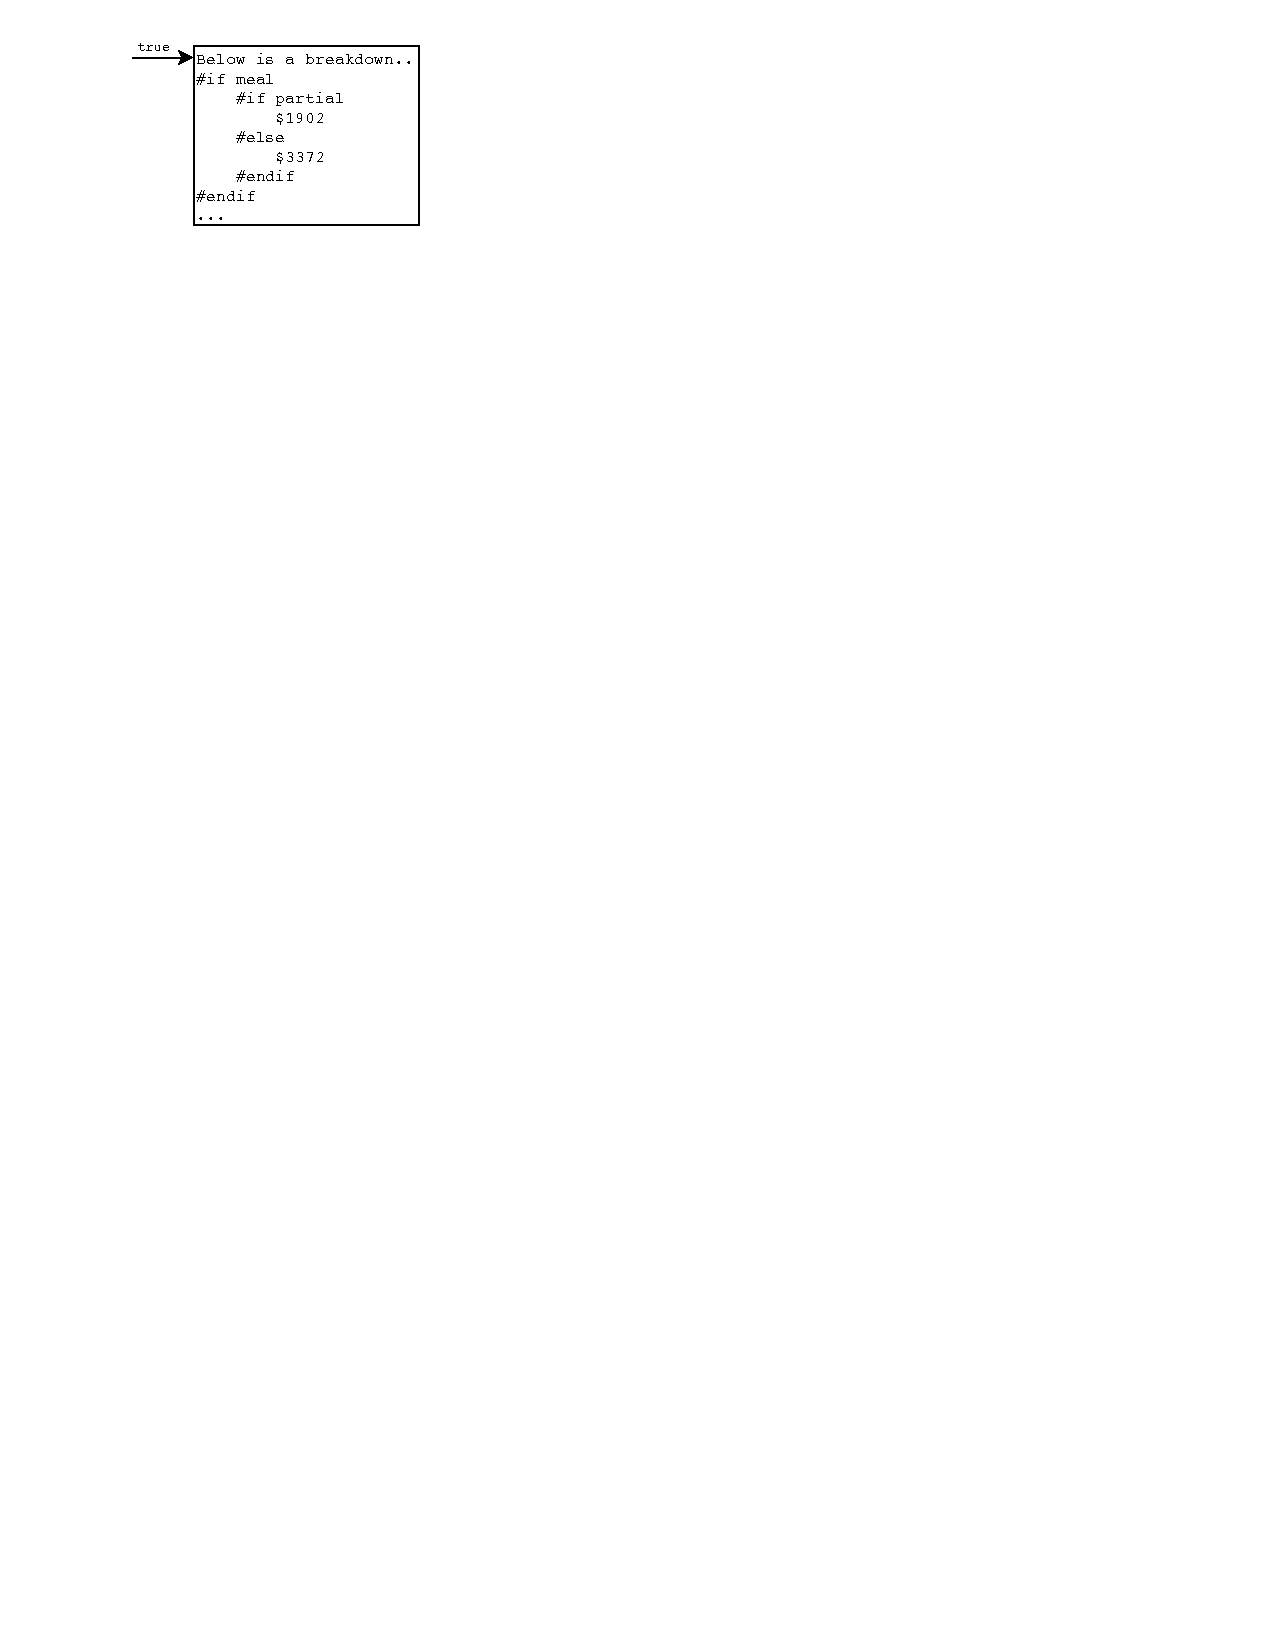
\includegraphics[scale=0.75]{figures/vfile-Page-1.pdf}
  \caption{Read-line in context \texttt{true}.}
  \label{fig:file1}
\end{subfigure}
\begin{subfigure}[b]{.33\textwidth}
  \centering
  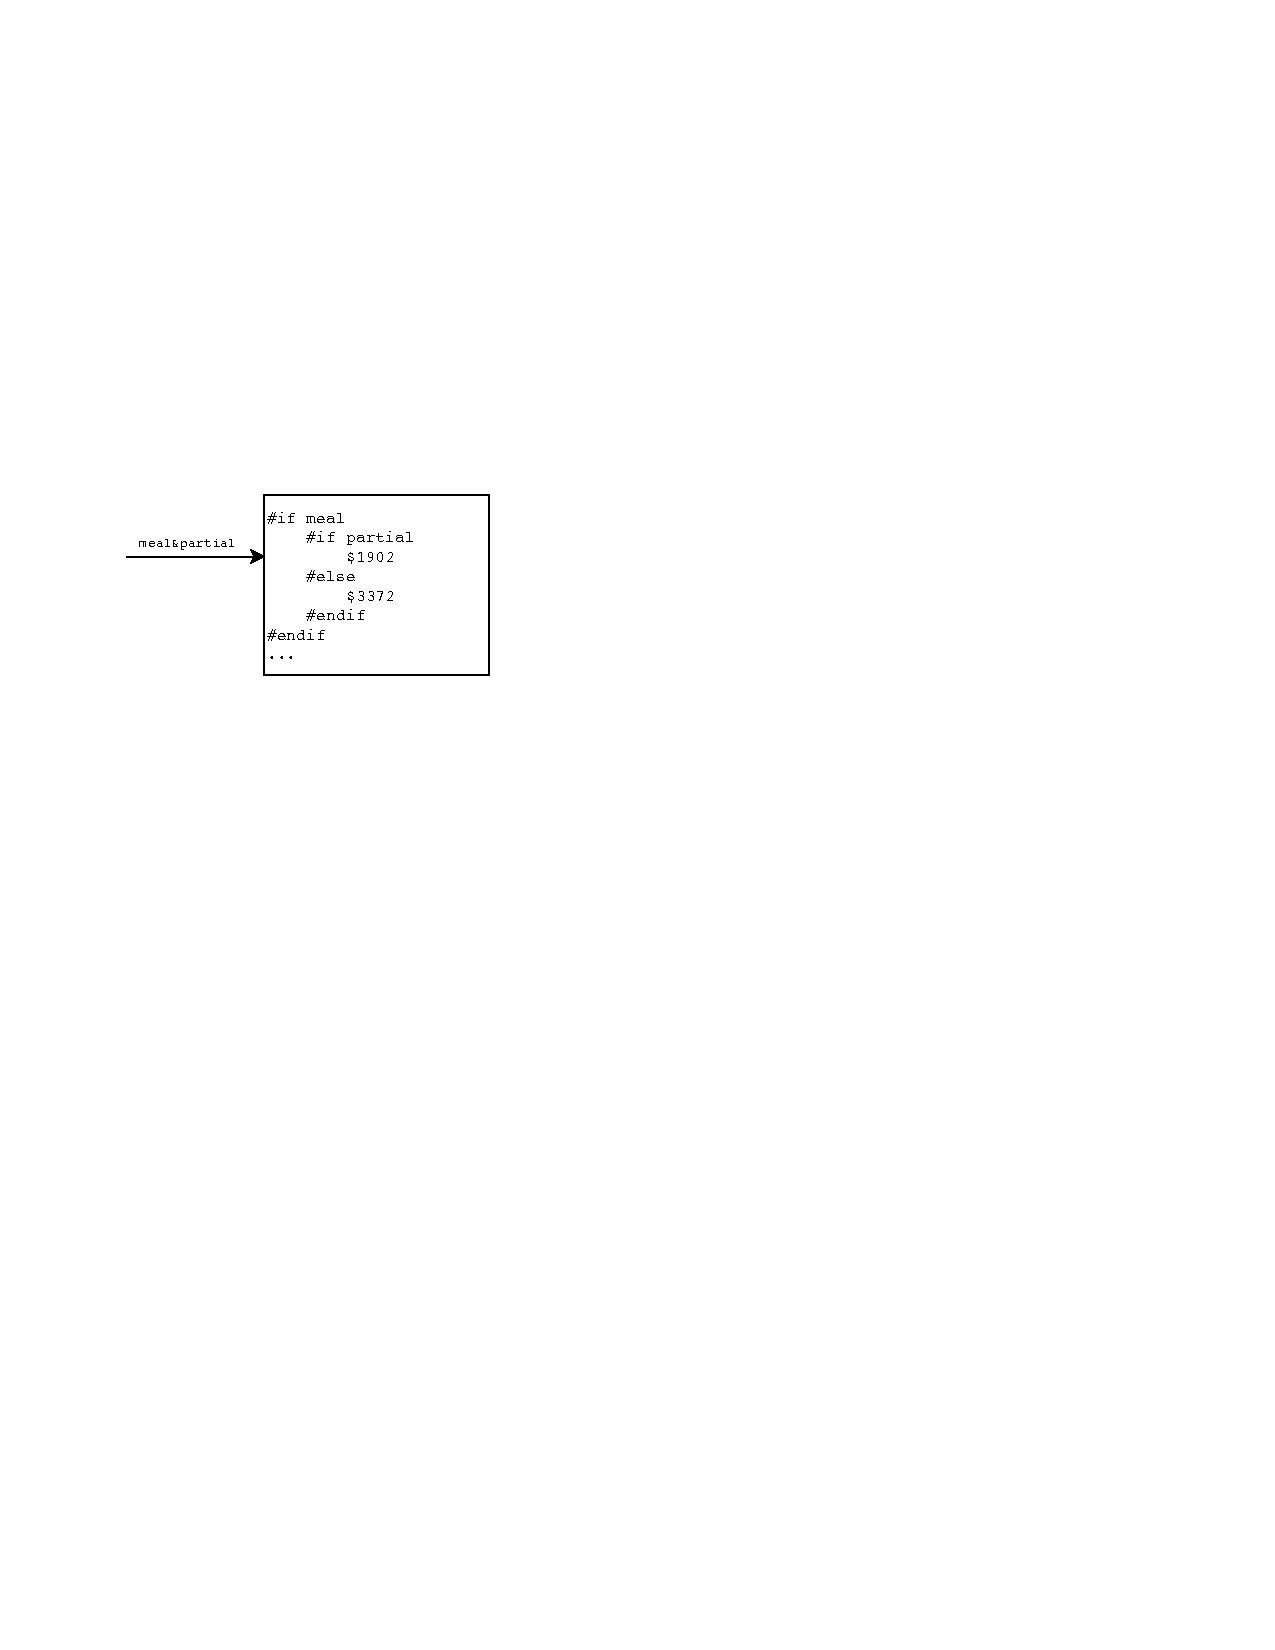
\includegraphics[scale=0.75]{figures/vfile-Page-2.pdf}
  \caption{Read-line in \texttt{meal\&partial}.}
  \label{fig:file2}
\end{subfigure}
\begin{subfigure}[b]{.33\textwidth}
\centering
  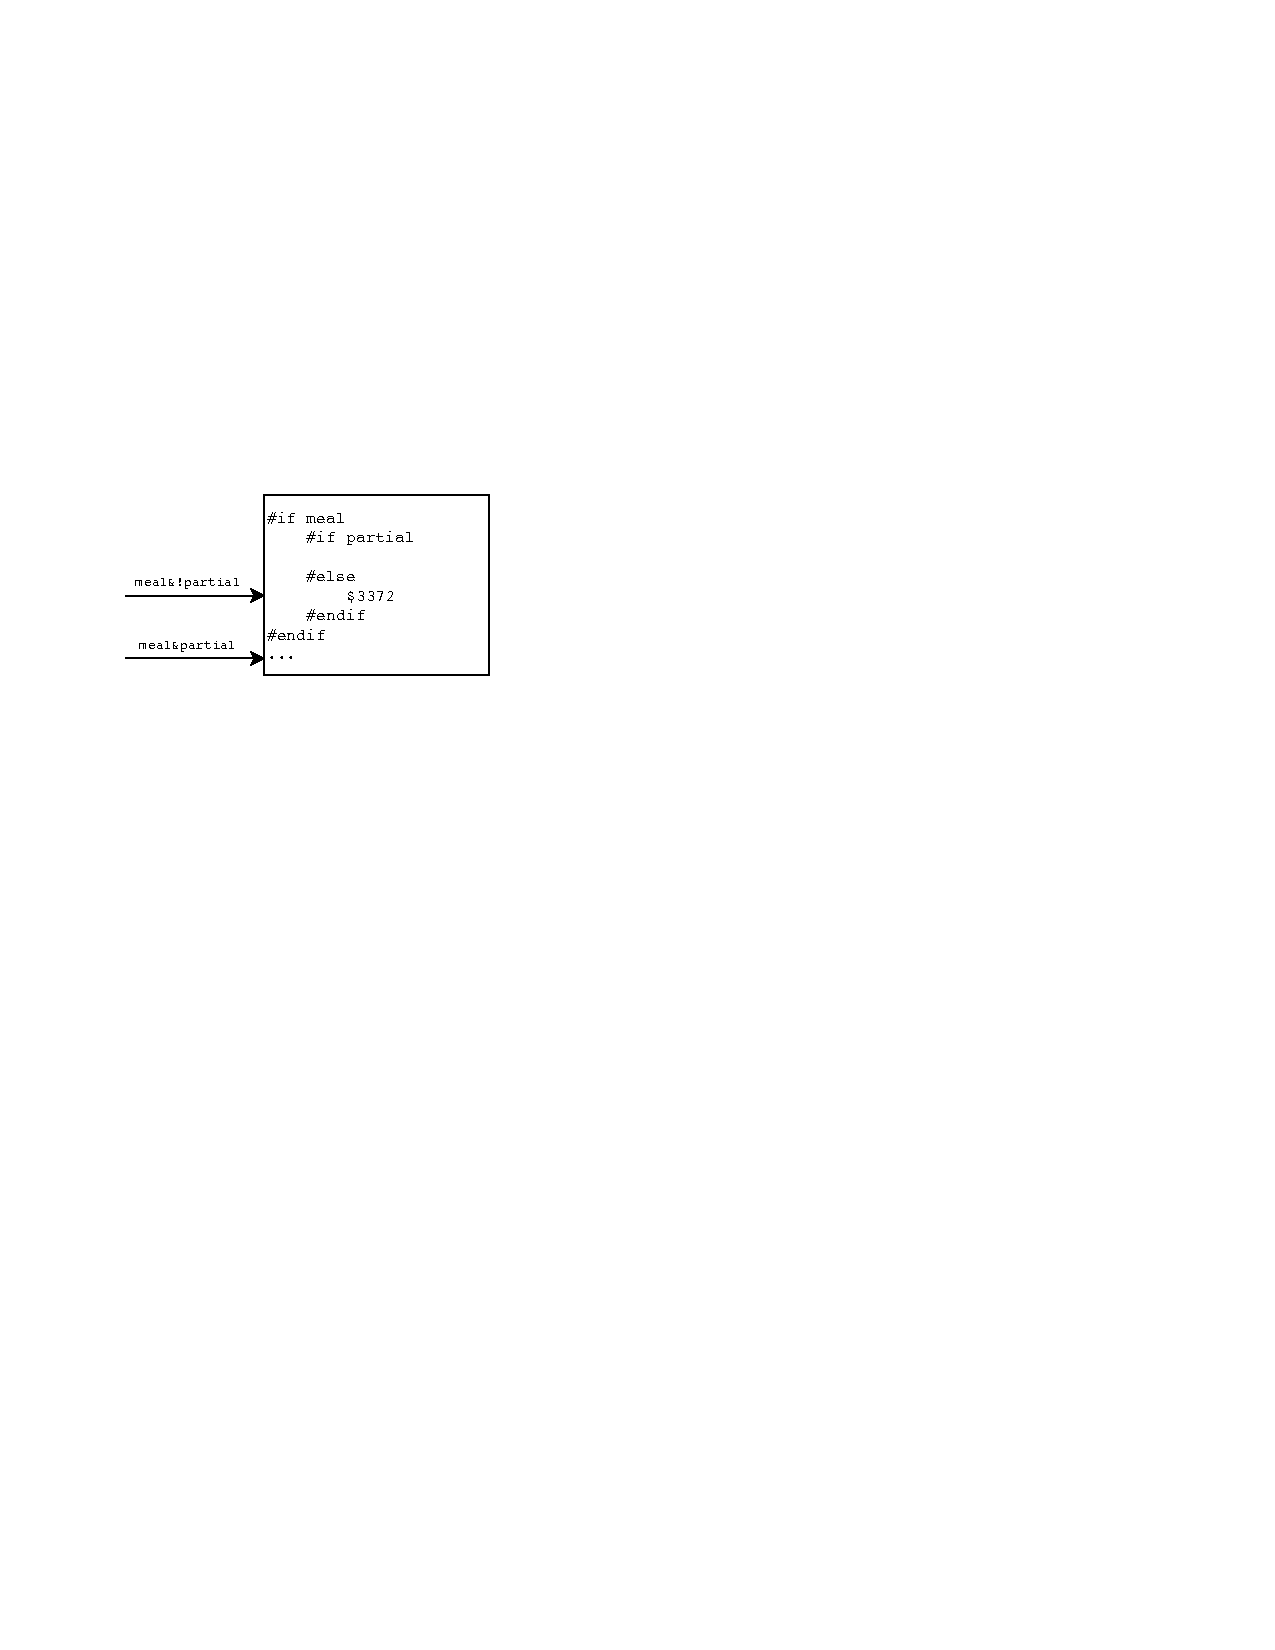
\includegraphics[scale=0.75]{figures/vfile-Page-3.pdf}
  \caption{Read-line in \texttt{meal\&!partial}.}
  \label{fig:file3}
\end{subfigure}
  \caption{File representation in a sequence of read-line operations.}
  \label{fig:file-figures}
\end{figure}
%

Plain read-line calls have context \texttt{true} by default. When we start to read from the file, the file pointer is at the first line of the file with context \texttt{true} as shown in Figure \ref{fig:file1}. We perform a read-line operation as shown below.
%
\begin{lstlisting}[escapeinside={(*}{*)}]
readLine file = "Below is a breakdown.." 
\end{lstlisting}
%
Reading in context \texttt{true} corresponds to reading from all file variants. Since the first line is plain, it is available in all variants, so we return it. 

We then perform a second read-line operation in the context \texttt{meal\&partial} as shown below.
%
\begin{lstlisting}[escapeinside={(*}{*)}]
(*$\Opt[\texttt{(meal\&partial)}]{\texttt{readLine file}}$*) = "$1902"
\end{lstlisting}
%
The file pointer now moves to the true alternative of the choice \texttt{partial} in line 2 as shown in Figure \ref{fig:file2} and we return the line \texttt{"\$1902"} corresponding to this context. 
%

We then perform a third read-line operation but in the context \texttt{meal\&!partial} as shown below.
%
\begin{lstlisting}[escapeinside={(*}{*)}]
(*$\Opt[\texttt{(meal\&!partial)}]{\texttt{readLine file}}$*) = "$3372"
\end{lstlisting}
%
We end up with two file pointers at two different locations. One with the context \texttt{meal\&!partial} pointing to the false alternative of the choice \texttt{partial} in line 2 and the other with context \texttt{meal\&partial} pointing to the third line as shown in Figure \ref{fig:file3}. We return the line \texttt{"\$3372"} corresponding to the context \texttt{meal\&!partial}. 

In the rest of this section, we show how we could manage these variational read-line calls and how we extend the environment to support file reading using algebraic effects. 

\section{Variational Queues for Representing Files}
\label{sec:queue_to_file}

We need to use a special data structure that could simulate the different plain files corresponding to different variation contexts in a variational file. Therefore, we use the variational queue implementation in Chapter \ref{sec:queue_lib} to represent files. This way we could load variational lines from the file into the queue using enqueue operations and read-lines from the file through dequeue operations. However, we still need to parse lines from the variational text file to be able to enqueue them.

In this section we show how to parse variational files into variational queues. The parser details are shown in Figure \ref{fig:parser}. The parser takes a variational text file as input and returns a variational queue as output. The queue is initialize to empty at the beginning. Parsing mainly occurs in the helper function \texttt{read}. The function \texttt{read} takes a file channel, queue, text and context as parameters. The text corresponds to the last line of text read from the file. The queue is updated with enqueue operations after parsing each line (plain or variational). The context corresponds to the context of a parent variational line if it exists; it is \texttt{true} by default.

%
\begin{figure}[h]
 \begin{lstlisting}
let rec read file q text ctx =

    if is_choice text then
        let ctx' = get_ctx text in 
        read_vline file q ctx ctx'
    else  
        enqueue' q text (Lit true)
        
and read_insert file q line ctx ctx'= 

    if is_choice line then 
        read file q line ctx'
    else 
        enqueue' q line (And (ctx',ctx)) 
				 
and read_vline file q ctx ctx' = 

    let line = get_next_line file in 
	
    if is_endif line then 
        q
    else if is_else line then 
        read_vline file q ctx (Not ctx')
    else
        let q' = read_insert file q line ctx ctx' in
        read_vline file q' ctx ctx'
;;
\end{lstlisting}
  \caption{Variational file parser.}
  \label{fig:parser}
\end{figure}

In the function \texttt{read}, we check if the text corresponds to a variational line by checking if it starts with the keyword \texttt{\#if}. If the text corresponds to a plain line, we directly enqueue it with context \texttt{true}. Otherwise, we parse the variational line in the helper function \texttt{read\_vline}. We pass two contexts as parameters: the context of the underlying choice (\texttt{ctx'}) and the context of any parent line (\texttt{ctx}).

In the helper function \texttt{read\_vline}, we read a line from the file, then determine in which variant of the variational line we are. If the line has the keyword \texttt{\#end}, we return the queue unchanged. If the line has the keyword \texttt{\#else}, we recursively invoke \texttt{read\_vline} with the negation of the context corresponding to the underlying choice (\texttt{ctx'}). Otherwise, we invoke the function \texttt{read\_insert}, which would insert the text of the underlying variant into the file. Then, we recursively invoke \texttt{read\_vline} again with the same context \texttt{ctx'} to parse the rest of the line. 

In the helper function \texttt{read\_insert}, we check if the variant has a nested variational line (choice). If there is a nested variational line, we recursively invoke \texttt{read} on it. Otherwise, we directly enqueue the line with its corresponding enqueue context. The corresponding enqueue context is the conjunction two context: the context of the parent variational line and the context of the underlying variational line. 


Besides parsing variational and plain lines, we also parse the contexts of variational lines. We show this parser code in the Appendix (Section \ref{sec:ctx_parser}).


\section{Variational Read-line}
\label{sec:file_read}

In this section, we write a new handler for the variation effect to support file reading and show an example of its use. We also show some useful applications of this work.

The handler \texttt{read\_v\_handler} in Figure \ref{fig:read-lib} allows us to perform read-line operations in variation. It also has a similar behavior to the variation handler in Figure \ref{fig:choice-impl} for handling the choice operations. However, in this handler we run the alternatives of the choice and return their corresponding results. In addition, we mange the variation context (or context for short), which helps separate the effects of the choice alternatives. With this implementation, we are able to determine in which alternative of the choice we are and thus figure out its corresponding context. The context is by default \texttt{true} with plain read-line operations. Otherwise, we use the operations \texttt{if\_}, \texttt{else\_}, and \texttt{end\_} to mange it.

\begin{figure}
\begin{subfigure}[b]{.5\textwidth}
  \centering
 \begin{lstlisting}[]
let if_ d =
    let (s,l) = #Get() in 
    let l' = (d :: l) in
    #Set((conjList l',l'))  
;;    

 let end_ () = 
    let (s,l) = #Get() in 
    match l with
        [] -> #Set((conjList l, l))
        | (x::l') -> #Set((conjList l', l'))  
;; 

\end{lstlisting}
\end{subfigure} \hspace{1em}
\begin{subfigure}[b]{.5\textwidth}
  \centering
 \begin{lstlisting}[]
let else_ () =
    let (s,l) = #Get() in 
    match l with
        [] -> #Set((conjList l,l))
        | (s':: l') -> 
            let s'' = (Not s') in 
            let l'' = (s''::l') in
            #Set((conjList l'', l'')) 
;;
  		
\end{lstlisting}
\end{subfigure}
  \caption{Operations for managing the variation context.}
  \label{fig:c-form-impl}
\end{figure}


\begin{figure}[!h]
 \begin{lstlisting}[]
let read_line f ctx = dequeue ctx f;;

let read_v_handler = handler
    | #Choice s k ->
        if_ s;
        let l = (k true) in
        else_ ();
        let r = (k false) in
        end_ ();
        (Chc (s,l,r))
    | #Read_line _ k -> k "c"
    | val x -> 
        if (is_empty x) then 
            Hole
        else 
            let q = #GetQueue() in
            let (c,_) = #Get() in
            let (r,q') = read_line q c in
            #SetQueue(q');  
            r
;;

let readLine () = #Read_line dfile;;

let read_line_h f = 
    with read_var_line_handler handle
        f ()
;;

let opt d t = chc d t "";;
\end{lstlisting}
\caption{File reading library.}
\label{fig:read-lib}
\end{figure}

The variation context is implemented as a mutable state (the algebraic effect and handler definitions for state are discussed in Section \ref{sec:background}) that holds a stack of contexts. To make things easier, we also hold the current context in the state making a tuple of two arguments: the current context and the stack of contexts. The entire implementation is shown in Figure \ref{fig:c-form-impl}. The first operation \texttt{if\_} takes a boolean formula over options and pushes it into the stack of contexts. The second operation \texttt{else\_} pops the top element (a context) of the stack and pushes the negation of it into the stack. The third operation \texttt{end\_} pops the top element (a context) of the stack. In every case after updating the stack of contexts, we update the current context to be the conjunction of all contexts in the stack.

Besides the variation context, we also manage another state in this handler which holds the variational queue representing the file. We choose to hold it in the state to avoid passing it between read-line operations. 

For catching the built-in effect operation \texttt{\#Read\_line}, which has a return type of string, we simply keep the continuation running with a default string. Note that we can neglect passing the file in every call to \texttt{\#Read\_line} and use a default file instead because the corresponding file representation is already passed to the handler. 

In the return case, we retrieve from the states both the variation context and the variational queue (representing the file). Then, we perform the \texttt{read\_line} operation on the file with the given variation context. The operation \texttt{read\_line} is basically a dequeue operation on the variational queue, which takes the variation context as parameter. The result of performing dequeue is a tuple of two arguments: the resulted line and the updated variational queue. The state holding the queue is set to the new queue \texttt{q'} and the result \texttt{r} is returned. Note that the return value of \texttt{read\_line} has type \texttt{v} because the result is either a plain line of text (\texttt{One}), a variational line (\texttt{Chc}), or nothing (\texttt{Hole}). 

Using this mechanism, we could read lines from variational or plain files, as shown below. 
%
\begin{lstlisting}[escapeinside={(*}{*)}]
let r_file = #Open_in "file.eff" ;;
let queue = read_v r_file;;
#Close_in r_file;;

let line1 () = readLine () ;;
let line2 () = (*$ \Opt[\texttt{(meal\&partial)}]{\texttt{readLine () }} $*);;
let line3 () = (*$ \Opt[\texttt{(meal\&!partial)}]{\texttt{readLine ()}} $*);;

let f () =
	read_line_h line1 ; read_line_h line2 ; read_line_h line3
;;

read_lines_h queue f;;
\end{lstlisting}
%
We open the file and then load it in a variational queue using the operation \texttt{read\_v} which is a parser explain in Section \ref{sec:queue_to_file}. After that, the file could be closed because the queue would be used instead to represent the file. The helper function \texttt{read\_line\_h} is used to wrap syntax of the variational read handler. The operation \texttt{read\_lines\_h} is used to wrap the syntax of states' handlers (variational queue state and variation context state). The example above shows the same sequence of read-line operations in Figure \ref{fig:file-figures}.

Because the results from read-line could be variational, we combine our work in file reading and variation to concatenate lines. 
%
\begin{lstlisting}[escapeinside={(*}{*)}]
let line1 () = readLine ();;
let line2 () = (*$ \Opt[\texttt{meal}]{\texttt{readLine ()}} $*);;

let g () =
    let res1 = read_line_h line1 in 
    let res1 = read_line_h line2 in 
    let r () = 
        let a1 = reflect_v res1 in
        let a2 = reflect_v res1 in
        a1 ^ "  " ^ a2 
    in reify_v r 
;;

read_lines queue g;;
\end{lstlisting}
%
We use the \term{reify} and \term{reflect} technique, which are the inverse of each other, to accomplish that. In reflect, we convert the \texttt{v} type result into a choice effect operation and in reify, we calculate the corresponding variational result using the variation handler in Figure \ref{fig:choice-impl}. The example above concatenates the results of two read-line operations. The first is a plain read-line operation and the second is a variational read-line operation with the context \texttt{meal}.
The result \texttt{a1} is a plain line of text while the result \texttt{a2} is a choice as shown below.  
%
\begin{lstlisting}[escapeinside={(*}{*)}, backgroundcolor = \color{lightgray}]
a1 = (*\texttt{"Below is a breakdown of the preliminary housing costs for 2018-2019."} *)
a2 = (*\Chc[\texttt{partial}] {\texttt{"\$1902"} }{\text{"\$3372"}} *) 
\end{lstlisting}
%
Therefore, the final result of concatenating the lines above is the following variational value.
%
\begin{lstlisting}[escapeinside={(*}{*)}, backgroundcolor = \color{lightgray}]
(*\Chc[\texttt{partial}] {\texttt{"Below is a breakdown of ..  \$1902"}}{\texttt{"Below is a breakdown of ..  \$3372"}} *)
\end{lstlisting}
%
This implementation enables us to see the results corresponding to different variants in one run of the program. 

The next example is another useful application that shows how the integration of variation and side effects can prevent from repetitive work. Being able to read all alternatives of the file at once, allows performing a filter operation on all alternatives at one run and getting the variational value of all alternatives. The following program counts the number of times the text "\$13360" occurs in any alternative of the variational file. 
%
\begin{lstlisting}[]
let checkDocs w q =
  let words = concatMap (fun str -> split str x) q in
  let matches = filter (fun a -> a = w) words in
  length matches
;;
			
let q' () = map (fun v -> (reflect_v v)) q in
let f ()  = checkDocs "$13360" (q' ()) in
reify_v f ;;

\end{lstlisting}

In a similar manner, we run a map operation converting every line to a choice operation (reflect). Then, we calculate the variational result using the variation handler (reify). In each alternative, we run the filter operation \texttt{checkDocs}. Running this program on the example file in Figure \ref{fig:file_example} will result \texttt{2} when the two expressions (\texttt{artists' residence \& (single | efficiency)}) and (\texttt{smith \& (!kitchen \& single)}) are true, \texttt{1} when only one of them is true, and \texttt{0} when both are false. The following choice represents the result (we use artists instead of artists' residence for short).
%
\begin{lstlisting}[numbersep=6pt, escapeinside={(*}{*)}, backgroundcolor = \color{lightgray}]
(*\Chc[\texttt{(artists\&(single|efficiency))}]{\Chc[\texttt{(smith\&!kitchen\&single)}]{2}{1}}{\Chc[\texttt{(smith\&!kitchen\&single)}]{1}{0}} *)
\end{lstlisting}




% In \texttt{read}, if the line was a plain text, it is inserted into the stack with the context \texttt{true} (line 25). If the line was variational (choice), the parser runs the algorithm below (line 22-23). The algorithm is almost identical for the left and right alternatives of the choice and shown in the helper function \texttt{read\_vline}. To indicate in which alternative we are, we pass the variable \texttt{fileCtx} which is either \texttt{L} or \texttt{R}. We start running this algorithm in the left alternative (\texttt{L}). 

% \begin{enumerate}

% \item (Line 4): to avoid getting into the end of file (eof), \texttt{get\_maybe\_next\_line} checks the maybe type line that was passed to the function. If the line has been read already, the line is wrapped in a \texttt{Just} constructor. Otherwise, \texttt{Nothing} is passed, which indicates that we should read the next line from the file. 

% \item (Lines 5-6): we first check if the line has the keyword \texttt{\#end} which happens in the case where there is an empty string in the else branch. If so, we return an empty list. Otherwise, we do the next steps. 

% \item (Lines 8-12): to find the next line to be returned (\texttt{next\_return\_line}), we check whether or not the line we are processing is a sub-choice. If it is so, we have to recursively call \texttt{read} to parse the sub-choice. Otherwise, we return the plain line from step 1. 

% \item (Line 12): the context of the line we return differs based on the value of \texttt{fileCtx} (\texttt{L} | \texttt{R}). If we are in the left alternative (\texttt{L}), the context stays the same. If we are in the right alternative (\texttt{R}), the context is negated. This is done int the function \texttt{upd\_ctx}.

% \item (Line 10): for sub-choices, the context is the conjunction of the updated context in the previous step and the context of the parent choice. This is done int the function \texttt{calc\_ctx}. 

% \item (Lines 15-20): after figuring out the next return line, we check if there is a keyword next, which guides to the next step. 
% \begin{itemize}

% \item (Lines 15-16): If we found the keyword \texttt{end}, we return the next return line from step 3.
% \item (Lines 17-18): if we found the keyword \texttt{else}, we repeat the algorithm but with the \texttt{fileCtx} (\texttt{R}) parsing the right alternative of the choice. We concatenate that with next return line from step 3.
% \item (Lines 19-20): if we found no keyword, we repeat the algorithm in the same alternative because having no keywords indicates that there are more lines of text in the same alternative. We concatenate that with next return line from step 3.
% \end{itemize}

% \end{enumerate}

\chapter{Limitations of Variation as an Effect}
\label{sec:efficiency}
% In this section, we address the challenges and concerns related to our work. 
Our choice effect is closely related to similar choice effects described in previous work on algebraic effects \cite{BP15effects,Pretnar15,Kammar2013,Plotkin2001}. The main difference is that our choices also include a formula that can be used to coordinate choices in different parts of the program. However, both are work and previous work share a common limitation: choices implemented as effects are very inefficient compared to built-in language support for variation.

One of the core ideas underlying variational execution is that parts of the program shared among two or more variants are executed only once. However, this is unfortunately not the case for variation implemented via choice effects. 

Consider the program below executing a variational list of numbers. 
%
\begin{lstlisting}[escapeinside={(*}{*)}]
with v_handler handle
    [5;9;7;(*\Chc[\texttt{B}]{\texttt{5}}{\texttt{6}}*);(*\Chc[\texttt{A}]{\texttt{11}}{\texttt{10}}*)] 
;;
\end{lstlisting}
%
Ideally, we would like the raw elements to be visited once: elements 5, 9 and 7. Now consider doing an operational computation on this list such as summing up the list. To figure out how many times every element in the list gets executed in calculating the sum, we use a state counter. This counter is incremented every time an element is visited as follows in \texttt{sum}.     
%
\begin{lstlisting}[escapeinside={(*}{*)}]
let rec sum l = 
    match l with 
        [] -> 0
        | (x::xs) -> #Set(#Get()+1); x + sum xs
;;
\end{lstlisting}
%
We return the sum of the list along with the value of the state counter as follows.
%
\begin{lstlisting}[escapeinside={(*}{*)}]
with state handle
    with v_handler handle
        let l = [5;9;7;(*\Chc[\texttt{B}]{\texttt{5}}{\texttt{6}}*);(*\Chc[\texttt{A}]{\texttt{11}}{\texttt{10}}*)] in
        (sum l, #Get())
;;
\end{lstlisting}
%
Because this lists has 4 variants, every element in the list has been visited 4 times. The program above outputted the following result. 
%
\begin{lstlisting}[escapeinside={(*}{*)}, backgroundcolor = \color{lightgray}]
[(A & B, (37,5));
((*$\neg$*)A & B, (36,10));
(A & (*$\neg$*)B, (38,15));
((*$\neg$*)A & (*$\neg$*)B, (37,20))]
\end{lstlisting}
%
This means that the size of the computation increases exponentially with respect to the number of options in the program; $ O(2^n)$. Unfortunately, we are not able to avoid this with the current approach, while it could've been more efficient to visit the list once until reaching the first variational element. The work in \cite{MMWWK17vamos} deals with this issue by designing multiple variational stacks' implementations that avoid repeating shared parts. However, doing this for every kind of variation we deal with is overwhelming. 


In this work, we chose to implement variational execution via choice effects for expediency. Our goal is to demonstrate how algebraic effects can be used to solve the problem of managing side effects during variational execution. However, a proper language for variational execution with side effects should include both algebraic effects and built-in support for variation. That is, built-in constructs for choices and optional values, and corresponding language run-time support for variational execution. 

The language \emph{Eff} we use to implement this work is an under development language, which makes this work more challenging. Its lack of features forces us to implement a basic incremental SAT solver to solve boolean formulas in our choices' contexts. If the language was more advanced with features, we could use a more efficient solver. Moreover, the language is lacking operations for file I/O and string manipulation features needed in paring. This also forces us to alter the type system to introduce new types such as \texttt{Channel} and \texttt{Char}, import various string operations from \emph{OCaml} and build a new compiler instance to work with. 


\chapter{Related Work}
\label{sec:rw}
In this section we discuss various related work. We briefly discuss a work that addresses the problem of integrating variation with side effects but does not solve it. We review in details a work that approaches the same problem we address and handles file I/O differently. Eventually, we compare our variation effect with the non-determinism effect. 

\section{VarexJ: A Variability-Aware Interpreter for Java Applications}

This work builds a virtual machine (VarexJ) for testing software product lines in variational settings allowing the testing of all configurations at one run \cite{Mein14:MS}. This machine has been successful in various aspects, but still suffers from the limitations of integrating side effects such as file I/O. 

In this work, they could not deal with files for testing in variation because the different configurations affect each other. For example, running the program to test with some configuration would read and write something to the file that would be changed or deleted when testing with another configuration. This could be managed with individual runs by resetting the file to the starting state, but with multi-execution software this is in-feasible as the result of one configuration might overwrite the other. Solutions suggested, but not implemented, to the problem include new file models, separating files for different variation contexts, or variability-aware file content encoding. 

\section{Typed Faceted Values for Secure Information Flow in Haskell}
\label{related_work2}
A major concern in programs that carry sensitive data is enforcing a policy that keeps the data safe and prevent attacks or unauthorized accesses to it \cite{Austin14,AF:POPL12}. A good strategy to control the information flow of the program is to require programmers to mark sensitive data to protect them. This has been effectively used to enforce information flow in secure multi-execution, where a program has two versions low and high. The high execution access and controls privates channels only, while the low execution controls public channels. The work in \cite{AF:POPL12} introduced faceted values to simulate both versions of the program in one process. The faceted value is equivalent to the choice in our work where one alternative holds the private facet and the other holds the public facet. However, these programs can still leak sensitive information through implicit flow when side effects are invoked. Therefore, the work in \cite{Austin14} extends on faceted values to make facet-aware I/O operations such as mutable references cells (mutable states) and socket communication through channels (file I/O).

Similar to our approach, they build a Haskell library that can be integrated into languages. They implement faceted values as monads separately from the side effects. Then, they extend them to work with side effects. Programs with side effects could be in the following form where \texttt{secret} is a faceted value. 
%
\begin{lstlisting}[escapeinside={(*}{*)}]
do v <- secret 
    do if v == 42 
        then writeIORef x 1
        else return ()
    readIORef x

\end{lstlisting}
%
This program in Haskell would have the type \texttt{(Facet (FIO a))} which can not be run (\texttt{FIO} is their limited version of \texttt{IO}). Therefore, their work converts programs of this type to the type \texttt{(FIO (Facet a))} to be able to run them soundly. In order for them to figure out the path of the program flow, they implement a program counter as a list denoting their selections (public or private) of the labels on faceted values used throughout the program. 

This implementation so far, has the same goal we have with the variation effect. However, we do not use a program counter to figure out the selections, we use the continuation which we invoke with true and false simulating all variants (variational execution). The return value of the continuation is the corresponded selection of the underlying choice label (option). 

% To create facet-aware reference cells, they implement an interface that works with the faceted types explicitly. The operations of it are similar to the state effect for writing, reading and initializing a new reference cell. For example, \texttt{readFIORef} has type \texttt{FIORef a -> FIO(Faceted a)}; it take an explicit faceted type of the cell and returns a faceted value. In our work however, we introduce new handlers and avoid introducing new effects. Our handlers catch the built-in effects and enforce new behaviors on them. This makes our work flexible and extendable by allowing us to handle the same effects in multiple ways. 

For file I/O and network sockets, they address the same issue we address that the file system or the channel have external environments that are not facet-aware. To make file I/O facet-aware, they introduce new operations that work with faceted values explicitly as shown below. 
%
\begin{lstlisting}[escapeinside={(*}{*)}]
openFileF :: View -> FilePath -> IOMode -> FIO FHandle
hGetCharF :: FHandle -> FIO (Faceted Char)
hPutCharF :: FHandle -> Faceted Char -> FIO ()
\end{lstlisting}
%
In our work however, we introduce new handlers and avoid introducing new effects. Our handlers catch the built-in effects and enforce new behaviors on them. This makes our work flexible and extensible by allowing us to handle the same effects in multiple ways. 

To avoid changing the external environment (the file system), they require raw data (either the public or private alternative) to be sent to the channel, or no data at all if the operation requires access to data that should not be accessed. Thus, the trick they use to work with file I/O on the library level is by attaching a view, which is a list of labels, to the file handle in \texttt{openFileF} operation indicating the privacy policy. 

The view attached to the handle is checked against the program counter, if the program counter selects a label that is not in the view, the underlying operations are disabled. Consider the following program with the program counter \texttt{["z","w","x"]}.
%
\begin{lstlisting}[escapeinside={(*}{*)}]
do h <- openFileF ["z","w"] "file" WriteMode
    hPutCharF h (makeFacets "z" 'a' 'b') 
\end{lstlisting}
%
No write should happen in this case to avoid leaking information to \texttt{"x"}, since it is not in the view. However, if the program counter was \texttt{["z"]}, character \texttt{'a'} would be written. 
%
Similarly, the read operation below is protected by the view holding \texttt{"k"} and \texttt{"l"}.
%
\begin{lstlisting}[escapeinside={(*}{*)}]
do h <- openFileF ["k","l"] "file" ReadMode
    hGetCharF h 
\end{lstlisting}
%
In comparison to our work, we extend text files with the CPP format which lets us control every line of the file and flexibly read and write variational lines from the file. On the other hand, they require all labels to be mentioned upfront when the file is opened.

The main property we maintain is the preservation property which ensures symmetry; one alternative of the choice does not control the other alternative. In contrast, their faceted values are asymmetric because the private alternative can control the public alternative, but the private alternative can not control the public alternative. Consider the example below. 

\begin{lstlisting}[escapeinside={(*}{*)}]
hPutCharh (*\Chc[\texttt{k}]{\texttt{'a'}}{\texttt{'b'}} *)
hGetChar h
\end{lstlisting}
%
Since only raw data could be sent to the file, either \texttt{'a'} or \texttt{'b'} could be written. If the user had access to the private alternative of \texttt{k}, the program would write \texttt{'a'} into the file. Then, the second line of code returns $\Chc[\texttt{k}]{\texttt{'a'}}{\_}$ to avoid information leak. While if the user had access to the public alternative of \texttt{k}, the program would write \texttt{'b'} into the file. Then, the second line of code returns \texttt{'b'} and not $\Chc[\texttt{k}]{\texttt{\_}}{\texttt{'b'}}$ which breaks the symmetry property. They claim that this approach is more natural and avoids the challenge of keeping track of all labels. 

\section{Algebraic Effects for a Non-deterministic Effect}
% \TODO{Following paragraph cut-and-pasted from ECOOP paper. Adapt and revise.}
Work on algebraic effects and effect handlers has frequently used a choice as an
example of a non-deterministic effect \cite{BP15effects,Pretnar15,Kammar2013,Plotkin2001}.  
These choice effects differ from our notion of choices in two key ways: (1)~Each choice effect is independent, there is no concept analogous to dimensions to synchronize selections across
choices. (2)~The evaluation of an expression with choice effects yields an
unstructured set of variants, rather than a structured variational value that clarifies
the relationship between a sequence of selections and the variant it yields, as
in our variation effect.
%
A notable exception is the \term{selection functional} effect presented in
\cite{BP15effects}, which essentially implements dimensioned choices in the
\emph{Eff} programming language.
%
However, the control flow enforced by these encodings of choices rules out
several ways to optimize variation-preserving computations. Since computations
for different alternatives are performed in different continuations, we lose
the opportunity to perform choice reduction to proactively eliminate
unreachable alternatives~\cite{CEW14toplas}, or to join converged execution paths early.

Finally, encoding choices as effects loses the ability to explicitly pattern match on them which is often needed for variational analyses. 

% This ability is often needed for variational analyses, for example, the ability to
% commute selections with computations is a critical transformation for analyzing
% software product lines~\cite{Kastner12:TCA,Kastner11:VPP,CEW12icfp,CEW14toplas,Apel10:TSF}.


\chapter{Conclusion and Future Work}
\label{sec:conc}
Integrating variation with side effects does not have a one-size-fits-all solution because each effect requires a special treatment and the solution for one effect might be incompatible with other effects. The best solution given the constraints is to solve this problem at the library level giving the programmer the tools to deal with the interaction of variation and effects. As a proof-of-concept, we use algebraic effects to encode variation as an effect. Then, extend the execution environment of variational programs to support file I/O. Algebraic effects allow programmers to handle new types of effects or handle the existing effects in multiple ways. This makes them highly complementary with variational programs. As part of our contribution, we implement an abstract variational queue, which is a variational data structure that could be used in many applications of variational programming to incorporate variational data collections. 

For future work, we could extend the execution environment of variational programs to handle new types of effects such as mutable states, standard input/output, and exceptions. We could also handle file I/O differently. For example, we could create a new file instance for every context initiated in the variational program. The name of every file instance corresponds to its context. We already showed a simulation of this in Chapter \ref{sec:introduction}. Our potential goal of this work is to include both algebraic effects and built-in support for variation in languages. That is, built-in constructs for choices and optional values, and corresponding language run-time support for variational execution. This would properly perform variational execution with side effects.

% The library is an extension to the languages and could be further advanced to deal with more effects on a case-by-case basis. This paper presents a proof-of-concept prototype for integrating variation with side effects in file I/O. We use algebraic effects and handlers to implement this work. We encode variation as an effect. Then, extend the library with new handlers that work with file I/O reading and writing. This makes our work orthogonal because the language is independent of its exertions. For example, the variation effect stands on its own without the effect-aware extensions, and so on. This work presents the basic idea that could be done for other types of effects. To make this work in file I/O more powerful and to keep the preservation property hold, we introduced a new file format that extends the plain file format with variation. Other work in \cite{Austin14} has dealt with the integration of variation and file I/O without altering the files. However, this makes their work more limited and breaks the preservation property as discussed in Section \ref{related_work2}. We hope that our proposed solution would be used in better settings to cope with the efficiency problems caused by the limited features of the language \emph{Eff} and the fact that variation is implemented as an external library. If variation was built-in into the language, we could design better ways to improve efficiency in variational programs.

\pagebreak

\bibliography{c/eric,c/martin,c/change,c/vds,c/fp,c/error-reporting,c/misc,c/dblp2_short}
\bibliographystyle{plain}

\pagebreak

\appendix

\chapter{Parsing the Boolean Formula of a Choice}
\label{sec:ctx_parser}
\begin{lstlisting}
let rec getChoice_ split_string left = 
	
    let rec go xss left' = 
        match xss with 
            [] -> ((Lit false),[])
            | (x::xs) -> 
                if (x =  ")") then 
                    (left',xs)					
                else 
                    let (c',es') = (getChoice_ xss left') in 
                    go es' c'
    in 
    match split_string with 
        [] -> (left,[])
        | (e::es) -> 		
            if (e =  "(") then 
                go es left
            else if (e = "!") then 
                let (l',es') = getChoice_ es left in 
                (Not l',es')
            else if (e = "&") then 
                let (r',es') =  (getChoice_ es left) in 
                (And (left, r'), arr')
            else if (e = "|") then 
                let (r',es') =  (getChoice_ es left) in 
                (Or (left, r'),arr') 
            else 
                ((Ref e),es) 
;;

let rec get_choice split_string left = 
    let (c,l) =  getCh split_string left in
    match l with 
        [] -> c
        | _ -> get_choice l c
;;

let parse_choice split_string = 
    match split_string with 
        [] -> (Lit false)
        | (x::xs)-> get_choice xs (Lit true);; 
\end{lstlisting}

\end{document}

